%!TEX root=thesis.tex
\documentclass[thesis.tex]{subfiles}

\begin{document}

This thesis is about \emph{effective equations of motion} for solid particles suspended in fluid flows. In all but the simplest cases we are unable to directly compute the forces acting on a solid particle from first principles. The fundamental equations of fluid mechanics are too complicated, and even finding a numerical approximation with a computer is often too expensive.

But if we limit our scope to a particular physical situation, we may exploit its particular properties to simplify the calculations. With these simplifications we may find an effective equation of motion for the motion of the suspended particles. The effective equation is simpler, and therefore more useful, than the fundamental equations. The price for the simplicity is that they apply only within the limited scope. In this thesis we consider \emph{small} particles. I will make a precise definition of what small means later. For now think of small as the plankton in the oceans, not the shark, or the misty droplets in the clouds, not an airplane.

The effective equations of motion are used as building blocks in higher-level modeling. For example the effective force on a small sphere becomes a building block in a model of the droplets in a rain cloud, and the effective torque on a spheroid is used to model the order of fibers in a paper-making machine.

The technical centerpiece of this thesis is the calculation of an effective equation of motion, starting from the fundamental equations. This effective equation describes the rotation of a spheroid which is small, but finite. The motion of a finite particle is affected by inertia, and so is the motion of the surrounding fluid. The inertia affects the forces and torques acting on the particle. These effects are captured in our calculation. It is described in detail in \Secref{effective} in Part II, and the appended Papers~A-D.

The new effective equation generalises aspects of an earlier effective equation: the Jeffery equation \cite{jeffery1922}, which is valid for truly small particles that are not affected by inertia. In addition to this project I have also worked on two other projects which involve the Jeffery equation (Papers~E \& F.)

\section*{Disposition of this thesis}

The remainder of this thesis consists of an extended summary, and the appended papers.

You are now reading Part I, which continues in \Secref{motivation} with a motivation for our research.
In \Secref{background} I attempt to introduce our research to a reader without a strong technical background. Perhaps the reader is a new student, or a curious uncle of mine. But I hope that also an experienced reader may enjoy the text.
\Secref{prerequisites} is a technical introduction to the prerequisite concepts needed to understand this thesis. In particular I discuss the Jeffery equation and its solutions in some detail. 

Part II is where I present the original research contained in the appended papers. I give an ``executive summary'' of each project, including the context of the questions and the main results.

Part III contains some technical appendices. These are mainly intended as a reference for myself, future students and other researcher collegues.

Part IV contains the published papers A-F.


\chapter{Motivation}\label{sec:motivation}

The motion of small particles suspended in fluid flows is a fundamental research topic of interest in many branches of science, as well as for technical applications. In some cases it is the actual motion of the particles that is of interest. For example, in the atmospheric sciences the collisions and aggregation of small drops are important to the formation of rain \cite{devenish2012}. Similarly, in astronomy it is believed that the collisions of small dust grains lead eventually to the formation of planets in the accretion disk around a star \cite{wilkinson2008}. Another example is in marine biology, where the dynamics of small planktonic organisms swirled around by the ocean is fundamental in understanding their feeding and mating patterns \cite{guasto2012}. 

In other contexts the motion of the individual particle is of lesser interest. Instead its effects on the suspending fluid is the topic of study. The properties of so-called complex fluids, meaning fluids with suspended particles, are studied in the field of rheology. For instance, the ``ketchup effect'' (where ketchup is stuck in the bottle, and nothing happens, and then suddenly all the ketchup pours out at once, only to solidify again on the plate) exists because of how all the microscopic particles suspended in the liquid orient themselves \cite{bayod2008}. On a more serious note, the similarly sudden onset of landslides in clay soils is related to the complex fluid of water and clay particles \cite{coussot2002}. A fundamental question in rheology is how to relate the microscopic motion of the suspended particles to the macroscopic behaviour of the complex fluid.

In many circumstances it is important to consider the non-spherical shape of particles, and how they are oriented. For instance, the ash clouds from volcanic eruptions play an important role in the radiation budget of our planet, and therefore its climate \cite{mather2003}. The ash particles are non-spherical \cite{gasteiger2011}, and their shapes and orientations influence how light and energy is absorbed in the volcanic cloud \cite{dubovik2002}. Similarly, the orientation of non-spherical plankton influences the light propagation through the upper layers of the oceans, determining to which depth life-supporting photosynthesis is possible~\cite{marcos2011}. 

Despite their diversity, all the above examples share a basis in a fundamental question. How do particles respond to a given flow, and how does the flow in return respond to the presence of particles? The underlying goal of our research is to find an answer to this fundamental question.
But the mathematics of fluid dynamics have challenged physicists and mathematicians alike for several hundred years. Before moving on to the description of my work, I allow myself to digress into the story of a seemingly innocent question: what is the drag force on a perfect sphere moving with constant velocity through a still fluid?

Until the early 19th century the prevailing theory was the following: a moving sphere drags along some of the surrounding fluid in its motion, and the force upon the sphere is equal to the force required to drag along the extra weight. The force must then be dependent on the weight, or more precisely the density, of the fluid. But in 1829, Captain Sabine of the Royal Artillery performed detailed experiments with a pendulum in different gases \cite{sabine1829}. By observing the attenuation of the pendulum motion in both hydrogen gas and in air, he concluded beyond doubt that the damping force on the pendulum is not proportional to the density of the surrounding gas - there has to be another force.

It was George Gabriel Stokes who first computed the force on a \emph{slowly moving
%\footnote{In modern lingo: viscous flow, characterised by $\re \ll1$ and $\st\ll1$. }
} sphere due to the internal friction of the fluid \cite{stokes1851}. He found that the force depends on the ``index of friction'', which we today know as the kinematic viscosity of a fluid. From his calculation, Stokes immediately concluded that ``the apparent suspension of the clouds is mainly due to the internal friction of air'' \cite{stokes1851}.

%(Eq.~(127) in Ref.~\citenum{stokes1851}.) 
The \emph{Stokes drag force} remains a great success, and it correctly predicts the forces for slowly moving particles. But the question of how to correctly amend the Stokes drag force to account for slightly faster motion turned out to be surprisingly hard. The correction took around a century of hard work, and the invention of a new branch of mathematics \cite{veysey2007}. If we dare ask how to properly calculate the drag force on a particle moving quickly, in a curved path, and in a fluid which itself moves, the answer is still debated.

Meanwhile, the Stokes theory for slow motion has been extended to include both forces and torques on particles of any conceivable shape \cite{jeffery1922,brenner1974,kim1991}. Much of modern research on particles in fluid flows still rely directly on these well-known results.

In general, the fundamental equations of fluid mechanics, the Navier-Stokes equations, seem to describe the motion of fluids. But applying them requires tremendous efforts due to their sheer complexity. Today, a modern supercomputer can produce an approximate solution for some simplified cases, like a cubic meter of moderately turbulent air without particles. But many interesting problems, such as a real rain cloud with drops, are far out of reach for any computer in any foreseeable future.

One aim of theoretical fluid mechanics is to derive new, simpler, equations of motion to use in place of the fundamental equations. This is in essence what Stokes did in 1851 for slowly moving spheres. But the price of simplification is the loss of generality. Every new physical situation potentially requires a new equation. And each new equation has to be tested against experiments and direct numerical solution of the general equations.

In this thesis I first present a derivation (Papers~A-C) and validation (Paper D) of an effective equation of motion for the orientation of a spheroid in a simple shear flow. This equation of motion takes one step beyond the Stokes approximation of slow movements, at the expense of being valid precisely only for the simple shear flow. Why this trade-off is worthwhile is explained in this thesis.
Secondly, the two remaining papers appended to this thesis involve the Stokes (\citet{jeffery1922}) approximation for the angular motion of ellipsoids in linear flows. Paper~E is an experimental verification of the predicted angular motions in shear flow. Paper~F discusses the rotations of axisymmetric particles in turbulent flows.

\chapter{Background}\label{sec:background}

Every now and then I get the question ``what is it you do, anyway?'' Often enough the question is posed out of sheer politeness, and I can simply say ``Physics! Tiny particles, like plankton, they tumble in the oceans, and stuff.'' But sometimes the question is sincere, and I find it quite challenging to explain what I do. I may say that we calculate how non-spherical particles rotate in flows. But that is comparable to if I was designing a gearbox, and said that I work with cars. It is true, but not very helpful. 

The following is an attempt at a description which is readable and not too complicated, but still complicated enough to get a glimpse of the physics.

\section{Our field of study: particles in flows}\label{sec:context}

Where do particles go when I put them into a flow? Which way do they face? How fast do they spin? These are all valid questions, but they are unspecific. Of course the answers depend on whether the particle is an aircraft or a grain of particulate carbon soot, and whether the fluid is air or water. 

I will start with an elaboration on fluid physics, move to the question why we consider rigid particles specifically, then say something about the forces acting on the particles. This will naturally lead us to why we must consider ``small'' particles, which is not obvious from the outset. But let's start from the beginning.

\subsection*{Fluids}

Many physical systems around us are fluids. The air we breathe, the water we drink, the blood in our veins are all fluids. As a working definition we can think of a fluid as a system where the constituent molecules move around more or less freely. Sometimes they interact with each other and exchange some energy. These collisions give rise to what you perceive as friction. You know that syrup has more friction than water: if you pull a spoon through syrup, more of your energy is expended colliding molecules than if you were to pull the spoon through water. A measure of how often and how violently the molecules collide is the \emph{viscosity} of a fluid, and we say that syrup has higher viscosity than water. Now, it gets interesting when something else, for example a drop of oil or a particle, is added to the fluid. Consider dripping a drop of oil into water. Then what happens depends on how the water molecules interact with the oil molecules. As you probably have experienced, oil molecules prefer to stick together. Therefore the oil concentrates into a drop where as many oil molecules as possible may be neighbours with other oil molecules.

But so far, the above is a very qualitative, and you may rightly say naive, description of what happens. One could say that a fundamental problem of fluid physics is to figure out where all the different molecules go. From the detailed knowledge of every molecule we may proceed to deduce where the oil drop goes, and how fast, or if it perhaps breaks up, or maybe merges with another drop. However, making something useful out of this molecular picture is very difficult.
Just consider that in one litre of water there are about $10^{25}$ molecules (that is a one followed by 25 zeroes). In fact, we are not even particularly interested in the specific details of every molecule. We are interested in the macroscopic, observable world that is built up from all these molecules. Therefore this thesis is not at all concerned with the detailed motion of molecules, but I still wanted to start with this picture because sometimes it becomes important to remember the origin of the macroscopic motion.

%\todo{connect forward to chap's about noise, fokker-planckery}.

\subsection*{Fluid dynamics}

The discipline studying the macroscopic properties and motion of fluids is called fluid dynamics. Some typical quantities studied there are the fluid velocity and pressure. We can think of the velocity at a certain position in the fluid as the average velocity of all the molecules at that point. The pressure is the force per area an object in contact with the fluid experiences, due to the constant bombardment of molecules. Think for example of the forces in a bottle of soda. There are well-known equations called the Navier-Stokes equations that tell us the velocity and pressure at every point in space and time, provided that we can solve them. You can see them in \Eqnref{nsintro} on p.~\pageref{eqn:nsintro}. We will soon return to how this helps us, but first we must restrict ourselves to avoid a difficult hurdle.

Recall our example of a drop of oil in water. The switch from a molecular view to a fluid dynamical view presents a new problem: if we do not keep track of every molecule, we instead have to keep track of which points in space contain oil and which contain water. A boundary surface separates the two materials, and this boundary can deform over time as the oil drop changes shape. This sounds very complicated. Indeed, drop dynamics is a topic of its own, which this thesis does not intend to cover. Instead, this thesis concerns \emph{rigid particles}.

\subsection*{Rigid bodies}

A rigid body in physics is an object whose configuration can be described by the position of one point (usually the center-of-mass) and the rotation of the body around that point. Simply put: it cannot deform. The dynamics of a rigid body is described by Newton's laws. In particular, the center-of-mass motion is described by Newton's second law: the force $\ve F$ on a body equals its mass $m$ times its acceleration $\ve a$,
\begin{align*}
    \ve F = m\ve a.
\end{align*}
The above equation describes the movement of the center-of-mass, and there is a corresponding law for the rotation. Since this thesis concerns \emph{orientational dynamics} of particles, here is Newton's law for the rotation of a rigid body:
\begin{align*}
    \ve T = \ma I \ve \alpha.
\end{align*}
It says that the torque $\ve T$ on a rigid body equals its moment of inertia $\ma I$ (that's like the mass for rotations) times its angular acceleration $\ve \alpha$,
The two equations above are deceivingly simple-looking, but their solutions contain full knowledge of the motion of a rigid body. I state the equations here only to draw a conclusion: in order to extract all the information about the motion of a particle, we need to know both the force and the torque acting on the particle at all times.

There are many kinds of forces which can potentially act on a particle. For example there is gravity if the particle is heavy, or magnetic forces if the particle is magnetic. But for now we consider the forces on a particle due to the surrounding fluid, so called hydrodynamic forces. In everyday terms the hydrodynamic force is the drag, as experienced by the spoon you pull through syrup. Uneven drag over a body may also result in a hydrodynamic torque. For instance, turbulent air striking the wings of an aircraft will induce a torque which you feel as a rotational acceleration while the pilot compensates.

\subsection*{Hydrodynamic forces}

In order to find out what the force on a particle is, we need to know how the fluid around the particle behaves. And for that, we need to solve the Navier-Stokes equations of fluid dynamics around the particle. We imagine the fluid in some environment (in lingo: ``boundary conditions''), for example the air in a cloud, or liquid soap in a small pipe. A solution of the equations tells us the velocity and pressure of the fluid at any given point in space at any given time. If we have a solution, there is a mathematical recipe for how to extract the resulting forces and torques on a particle in the fluid.

The problem is that we cannot solve the equations. Not only are we unable to find solutions as mathematical formulas -- in many cases we can not even find numerical solutions using a supercomputer. For example, computing the motion of the air in a cloud is utterly out of reach with any computer we can currently imagine. Before moving on to how we find the force on a particle, I'll digress on the topic of numerical solutions.

From time to time I get the question why we struggle with difficult mathematical work, why not just ``run it through the computer?'' An answer to this question is that a numerical computer solution is like an experiment: it will give you the numbers for a particular case, but not necessarily any understanding of why. Conversely, we may extract physical understanding from the equations, even if we cannot solve them in general. It is the understanding of the underlying physics that enables us to simplify the equations until it is practical to solve them. This requires knowledge of which particular details may be neglected, and which details are crucial to keep track of. 
And indeed, the meteorologists now have methods of simulating the flows of air in the atmosphere, despite the fact that we cannot solve the exact equations. The trick is to ignore some parts of the equation dealing with very small motions, and spend the resources on describing the large eddies of the flow in so-called ``Large Eddy Simulations''.

At any rate, we wish to figure out what the forces on a rigid body in a fluid flow are. It is clear that some type of simplification has to be made, because we cannot solve the Navier-Stokes equations. The great simplification is embodied in the word \emph{small} in the title of this thesis. The particles we consider are small. But how small is a small particle? The answer I have to give right away is a rather unsatisfactory ``it depends''. The smallness of the particle has to be relative to something else. This simple principle is formalised by scientists, who discuss smallness in terms of \emph{dimensionless numbers}. Because dimensionless numbers are very common in our work I will spend a few paragraphs to explain the basic idea.

\subsection*{Dimensionless numbers}

In principle all physical quantities have some units. For example, the size of a particle has units of ``length'', and the speed of the particle has units of ``length per time'', which we write as \nobreak{length/time}. Whenever we multiply or divide quantities with units, we also multiply or divide their units. For example dividing the length \unit[20]{m} with the time \unit[5]{s} gives the speed \unit[4]{m/s}. Now suppose we divide the speed \unit[4]{m/s} with the speed \unit[2]{m/s}. The result is $2$, without any units -- they cancelled in the division.

The idea is that in order to determine if a quantity $x_1$ is ``small'' we have to divide it with another quantity $x_2$ of the same units. Then if the resulting dimensionless number $x_1/x_2$ is smaller than $1$, we say that $x_1$ is small, and implicitly mean \emph{relative to $x_2$}. This concept seems simple enough. Let's apply it to particles moving in a fluid.

\subsubsection*{An example: the particle Reynolds number}

Imagine stirring your cup of tea with a spoon. As you stir there is a wake behind the spoon, perhaps even a vortex is created if you are enthusiastic. When you stop stirring, the tea will splash about for a moment and then settle down because of its viscosity. If you stir vigorously, then stop suddenly and hold on to the spoon, you feel the force of the splashing fluid on the spoon. This continuing motion after you stopped forcing the fluid is due to the inertia of the fluid. Inertia means that things continue to move in their current direction, unless a force is applied. The inertia of the fluid is difficult to analyse mathematically, because the force on the spoon depends in a complicated fashion on how you stirred the tea in the past. To perform my calculation I want the inertia to be \emph{small}. But small compared to what? How can I make a dimensionless number?

Imagine stirring with a spoon in syrup instead of tea. The wake behind the spoon relaxes quickly in the more viscous fluid. The viscosity is the force which cancels the inertia. The viscous friction smears out any disturbances. Therefore we divide two times: the time it takes for viscosity to smear out a disturbance over the particle (the \emph{viscous time}), with the time it takes for the fluid to flow past the particle:
\begin{align*}
\rep = \frac{\textrm{Viscous time}}{\textrm{Time for fluid to flow past the particle}}.
\end{align*} 
This number is called the particle Reynolds number. It is small when inertia is not important.
If the viscous time is short, a disturbance is smeared out before it is allowed to flow past the particle. This is similar to stirring syrup. But if the fluid flows past the particle before the viscosity can smear out the disturbances, the particle Reynolds number is larger, like in your cup of tea.

The mathematical expression for the particle Reynolds number is 
\begin{align*}
	\rep = \frac{u_0 a}{\nu},
\end{align*}
where $u_0$ is the fluid velocity past the particle (units $\unit{m/s}$), $a$ is the particle size (units $\unit{m}$), and $\nu$ is the viscosity (units $\unit{m^2/s}$). This gives us three options to keep the effects of inertia small: consider slower flows, or smaller particles, or fluids with higher viscosity.  

Recall the story about the Stokes drag in the very beginning of this thesis. When Stokes in 1851 called a particle ``slowly moving'', he meant exactly the condition that the particle is small, in the sense just described here. Between friends we often say ``small particle'', or ``slowly moving'', or ``viscous flow'', when we mean ``small value of the particle Reynolds number.'' It is convenient, but less precise.

The reduction of three options into the value of a single number is an important insight. Instead of considering the effects of all three separate parameters, we can understand the physics by analysing a single dimensionless number. The dimensionless numbers tell us which physical quantities are important in relation to each other. In the example above, the actual size of the particle is not important -- the size only matters in relation to the velocity and viscosity. All situations with the same particle Reynolds number are, in some sense, equivalent. This very fact is also what enables engineers to use scale models in wind tunnels. They know that to test a model of a suspension bridge in a wind tunnel, they can not use full-scale wind speeds, but instead a scaled down version of the wind. The dimensionless numbers reveal what scaling is appropriate to match the model bridge to real conditions.
\subsection*{Conclusion}

We have discussed fluids, rigid particles, the Navier-Stokes equations and dimensionless numbers. If we add some mathematical rigor to the mix, you could soon have an undergraduate degree in fluid mechanics. But how does this connect to my research?

When we assume that there is no fluid inertia whatsoever, that is $\rep=0$, we enter the regime of the Stokes approximation. As explained in the introduction this approximation has been fantastically successful in predicting the forces and torques on particles in many situations. But for some special cases, the Stokes approximation does not lead to a definite answer. One of these cases is the rotation of a non-spherical particle in a so-called shear flow. Jeffery applied the Stokes approximation to this problem in 1922, and was disappointed to find that the answer is indeterminate. My contribution in this thesis is to amend the Stokes approximation for this particular case. The four Papers A-D explain the first effects of both fluid and particle inertia on the rotation of a non-spherical particle in shear flow.

During the course of this work, I have also worked with students and collegues on related problems. How does the particle rotate if we throw it into a turbulent fluid? Can we tune an experiment to match the Stokes approximation? These and many more questions are ongoing work, and we published some results in the Papers E \& F.

\chapter{Prerequisite concepts}\label{sec:prerequisites}

In this section I introduce some basic concepts needed to understand my work in Part II of this thesis, and the appended papers. My aim is to start at the beginning, and as quickly as possible arrive at the knowledge particular to the field of orientational dynamics of non-spherical particles. The scope is therefore narrow, but deep.

\section{Fluid mechanics}

\subsection{Fluid flows}\label{sec:fluidflows}

In this thesis we only encounter so-called Newtonian and incompressible fluids. The hydrodynamic state of such a fluid is described by a flow velocity vector field $\ve u(\ve x,t)$, and a scalar pressure field $p(\ve x, t)$. The incompressible nature of the fluid implies that $\nabla \cdot \ve u = 0$ everywhere.
The fluid itself has two properties: its density $\rho_f$ ($\unitfrac{kg}{m^3}$), and its dynamic viscosity $\mu$ ($\unitfrac{kg}{m\cdot s}$). Sometimes it is convenient to refer to the kinematic viscosity $\nu = \mu / \rho_f$ ($\unitfrac{m^2}{s}$).

The work presented in this thesis involve the flow gradients, because it is the gradients in the flow that gives rise to the torque on a small particle.

The spatial derivatives of the flow field $\ve u$ form a tensor $\ma A \equiv \nabla \ve u\transpose$, because there are three vector components defined in three coordinates. The components of $\ma A$ in cartesian coordinates are
\begin{align}
A_{ij}=\pdiff{u_i}{x_j}\,.	
\end{align}
In general $\ma A$ is defined as the directional derivative in the direction $\hat{\ve y}$:
\begin{align}
 	\ma A\hat{\ve y} = \lim_{\epsilon\to 0}\frac{\ve u(x+\epsilon \hat{\ve y},t)-\ve u(\ve x, t)}{\epsilon}\,.
\end{align}
The incompressibility condition $\nabla\cdot\ve u=0$ transfers directly to the condition $\tr \ma A=0$.

It turns out that it is almost always convenient to decompose the gradient tensor $\ma A$ into its symmetric part $\ma S$ and anti-symmetric  part $\ma O$:
\begin{align}
	\ma A = \ma S + \ma O,\qquad
	\ma S = \frac{1}{2}\left(\ma A + \ma A\transpose\right),\qquad
	\ma O = \frac{1}{2}\left(\ma A - \ma A\transpose\right)\,.
\end{align}
The symmetric part $\ma S$ is called the rate-of-strain tensor, and it describes the local rate of deformation of the flow. The anti-symmetric part $\ma O$ describes the local rotation of the flow and is related to the vorticity vector. The vorticity vector $\ve \omega_f$ of a flow $\ve u$ is defined by the curl $\ve \omega_f = \nabla \cross \ve u$. The matrix $\ma O$ is related to the vorticity vector $\ve \omega_f$, because for any given vector $\ve x$
\begin{align}
	\ma O \ve x &= \frac{1}{2}\ve \omega_f \cross \ve x \equiv \ve \Omega \cross \ve x.\eqnlab{vorticityOdef}
\end{align}
The vector $\ve \Omega=\ve \omega_f/2$ is a common quantitiy in our calculations, and therefore is given its own symbol.

\subsection{The Navier-Stokes equations}

For a given physical situation the flow and pressure fields are determined by a Navier-Stokes problem.
A Navier-Stokes problem for a Newtonian, incompressible fluid is fully specified by a momentum balance, the incompressibility condition and a set of boundary conditions.

Let us first derive the momentum equations. Consider the momentum balance in a volume $\mathcal V$ bounded by surface $\mathcal S$. I think of these as Newton's $m \ve a = \ve F$ over a volume:
\begin{align}
    \pdiff{}{t}\int_\mathcal V  \rho_f \ve u \rd\mathcal V +
    \int_\mathcal S \rho_f\ve u (\ve u \cdot \rd \mathcal S) =
    \int_\mathcal S \bbsigma \cdot \rd \mathcal S \eqnlab{nsderiv1}
\end{align}
The first term accounts for changing velocities in the bulk of the volume. The second term accounts for the momentum transfer across the boundary of the volume. The right hand side contains the forces acting on the surface of the volume. The stress tensor $\bbsigma$ describes the force per unit area in the fluid, such that $\bbsigma\cdot \ve N$ is the force per area on a surface with normal vector $\ve N$. A Newtonian fluid is modeled by $\bbsigma = -p \ma 1 + 2\mu \ma S$, meaning that the forces arise in part from pressure, and in part from the viscous friction forces. This tensor is central in determining the forces on particle surfaces, too, as will be explained below.

We apply the divergence theorem to the surface integrals in \Eqnref{nsderiv1} and find
\begin{align}
    \pdiff{}{t}\int_\mathcal V  \rho_f \ve u \rd\mathcal V +
    \int_\mathcal V  \left[(\nabla\cdot\rho_f\ve u) \ve u+(\rho_f\ve u\cdot\nabla) \ve u\right] \rd \mathcal V =
    \int_\mathcal V \nabla\cdot\bbsigma \rd \mathcal V.
\end{align}
This equation holds point-wise, because the volume can be arbitrarily chosen. By using the incompressibility condition, we arrive at the Navier-Stokes equations for an incompressible fluid:
\begin{align}\eqnlab{nsintro}
    \rho_f \left(\pdiff{}{t}\ve u + (\ve u \cdot \nabla) \ve u\right)=\nabla \cdot \bbsigma\,,\quad \nabla \cdot \ve u = 0\,,\quad \bbsigma = -p \ma 1 + 2\mu \ma S\,.
\end{align}
The boundary condition where the fluid meets a solid surface is the \emph{no-slip condition}. This means that the fluid at the boundary has the same velocity as the boundary itself. When considering problems with a particle suspended in a fluid, the typical boundary condition is no-slip on the particle surface and that the flow relaxes to a prescribed background flow as the distance to the particle goes to infinity. 

\subsection{Forces on particles}

Consider a background flow $\ve u^\infty(\ve x,y)$ without any particle present. We introduce a particle into the flow through the no-slip boundary conditions at the particle surface $S$. The particle center-of-mass moves along the trajectory $\ve y(t)$ (velocity $\dot{\ve y}$), and its orientation $\ma R(t)$ changes with angular velocity $\ve \omega(t)$.  Far away from the particle, ``at infinity'', the fluid is not disturbed by the presence of the particle, and should be equal to $\ve u^\infty(\ve x,t)$:
\begin{align}
    \ve u(\ve x, t) &= \dot{\ve y} + \ve \omega \cross (\ve x - \ve y), & \ve x \in S(\ve y, \ma R). \nn\\
    \ve u(\ve x, t) &= \ve u^\infty(\ve x, t), & |\ve x-\ve y|\to\infty\,.\eqnlab{nsbc}
\end{align}
As explained above, the hydrodynamic force on a surface in the fluid is determined by integrating the fluid stress tensor $\bbsigma$ over the surface. Therefore the forces and torques acting on the particle are
\begin{align}
    \ve F &= \int_S \bbsigma \cdot \rd \ve S\,, \nn\\
    \ve T &= \int_S (\ve x - \ve y) \cross \bbsigma \cdot \rd \ve S\,. \eqnlab{nsforces}
\end{align}
To complete the problem formulation, the particle trajectory is governed by Newton's equations
\begin{align}
    m\ddot{\ve y} = \ve F\,, \quad \diff{}{t}(\ma I \ve \omega) = \ve T\,. \eqnlab{newtons}
\end{align}
Here $m$ is the particle mass, and $\ma I$ its moment-of-inertia tensor.

The coupled equations (\ref{eqn:nsintro}-\ref{eqn:newtons}) describe the motion of both particle and fluid. However, they are incredibly complicated because of their non-linearities: the so-called \emph{convective term} $(\ve u \cdot \nabla) \ve u$ in \Eqnref{nsintro}, and the coupling through the moving boundary conditions \eqnref{nsbc}.

We may understand that the problem is very hard just by imagining a particle in a fluid: as the particle moves and rotates, it stirs up a wake and vortices in its trail. These disturbances may linger and affect the particle at a later time. It seems that we are, in general, obliged to take into account the whole joint history of the particle and the fluid to predict the final state of the two. These complications raise the need for approximation, and \emph{effective equations} for the particle motion.

\section{Effective equations of motion}

For the purposes of this thesis, the term \emph{effective equations of motion} means a set of equations for the particle motion that does not involve the equations of fluid motion. The effective equations should be an approximation to the exact equations (\ref{eqn:nsintro}-\ref{eqn:newtons}) in some limit.

In principle that means that the force on the particle is a function of the particle state and history, and the background flow field $\ve u^\infty$:
\begin{align}
	\ve F_{\mathrm{eff}} &= \ve g(\ve y, \dot{\ve y}, \ma R, \ve \omega, \ve u^\infty)\,.
\end{align}
A concrete and well-known example is the Stokes force on a spherical particle of radius $a$
\begin{align}
	\ve F_{\mathrm{Stokes}} &= 6\pi\mu a (\ve u^\infty(\ve y, t)-\dot{\ve y})\,,\eqnlab{stokesforce}
\end{align}
which we will discuss in detail shortly.

The effective equation is also called a \emph{one-way coupling} approximation, because it explicitly gives the effect of the fluid on the particle, but not the other way around. We can therefore first compute, or choose, a flow field $\ve u^\infty$ in absence of any particles, and then use the effective equation to calculate the particle motion. This is a great simplification over solving the exact coupled system. It is a very common method to study for example the motion of particles in turbulence (for example, in Paper~G).

But we have to be careful. In the derivation of the Stokes force, it is assumed that the particle is alone in the fluid. If we use the Stokes force to consider several particles simultaneously and they happen to move close to each other, the approximation is no longer valid. In that case, we must create an effective equation for the particle pair instead. If the particle moves close to a wall, we have to make yet another equation for that. The price of simplicity is specialization.

\subsection{The particle Reynolds number}

My specialization is the the effective equations valid for ``small'' particles. The Stokes force in \Eqnref{stokesforce} was derived in 1851 \cite{stokes1851} and is the first example of this specialization. Let me make explain this limit more precisely.

As explained above, a particle moving through a fluid creates disturbances that may come back and affect the particle at a later time. We are aiming for the limit where the disturbances will be smeared out by the viscosity before they make any secondary impact. This happens if the time for viscosity to smoothen the flow field is smaller than the time it takes for the flow field to transport the disturbance over the particle size. The condition is precisely that the dimensionless particle Reynolds number is small. As stated in Sec.~\ref{sec:context},
\begin{align}
 	\rep = \frac{\textrm{Viscous time}}{\textrm{Time for fluid to flow one particle length}}.
\end{align}
More specifically,
\begin{align}
	\rep = \frac{a^2/\nu}{a/u_0} = \frac{u_0 a}{\nu},
\end{align}
where $u_0$ is a typical flow speed relative to the particle surface, $a$ is the size of the particle and $\nu$ is the kinematic viscosity of the fluid. We see that the limit I call ``small particles'' is actually that of either small particles, or large viscosity, or slow motions. The Reynolds number determines whether the inertia of the fluid is important compared to the viscosity.

In my work on rotating particles in shear flows, the typical flow speed $u_0 = sa$, where $s$ is the shear rate (the shear flow is explained in detail in \Secref{shearflow}.) The resulting dimensionless number is sometimes called the shear Reynolds number
\begin{align}
	\Reys = \frac{sa^2}{\nu}\,.
\end{align}
We introduce the dimensionless numbers in our equations by changing all variables into dimensionless variables using the available dimensions of the problem: length $a$ and time $1/s$. In my case the change of variables is $\ve u = sa \ve u'$, $p=\mu s p'$, $\ve x= a\ve x'$, and $t=t'/s$. We make this change in \Eqnref{nsintro}, drop the primes, and find
\begin{align}
\Reys \left(\pdiff{}{t}\ve u + (\ve u \cdot \nabla) \ve u\right)=\nabla \cdot \bbsigma\,,\quad \nabla \cdot \ve u = 0\,,\quad \bbsigma = -p \ma 1 + 2\ma S\,.\eqnlab{nsintrodimless}
\end{align}
In the limit of $\Reys\to 0$ we can hope to compute the force and torque on a particle by perturbation theory. The Stokes approximation is to set $\Reys=0$, and solve $\nabla \cdot \bbsigma=0$. This important limit is the topic of \Secref{stokes}.
\subsection{The Stokes number}\label{sec:stokesnumber}
If we change the variables in the fluid equations, we must also make the corresponding changes in the coupled particle equations. The equation for the angular dynamics, for instance, becomes\footnote{I am sweeping some finer details under the carpet here. They are irrelevant for this argument, and you'll find it all in Sec.~III in Paper C.}
\begin{align}
	\st\diff{}{t}(\ma I \ve \omega) = \ve T\,,\quad  \st= \frac{\rho_p}{\rho_f}\Reys\,.
\end{align}
Another dimensionless number shows up: the Stokes number $\st$. The Stokes number determines whether the particle inertia is important compared to the fluid forces. It is therefore not surprising that the Stokes number is related to the particle Reynolds number. They both compare inertial effects to the viscous forces. The only difference is through their relative densities. If the particle is heavier, its inertia is more important than the inertia of the fluid, and vice versa. 

A neutrally buoyant particle has the same density as the fluid: $\rho_p = \rho_f$, and $\st = \Reys$. This means that when we assume $\Reys$ small, we also assume $\st$ small. If the densities are different, we must consider the effects of gravity, unless $\Reys=\st=0$. In this thesis I don't consider the effects of gravity, and therefore $\st = \Reys$.

\section{The Stokes approximation}\label{sec:stokes}

In the extreme case when $\Reys=0$, the Navier-Stokes equation \eqnref{nsintrodimless} reduces to the linear Stokes equation $\nabla \cdot \bbsigma = 0$:
\begin{align}
	\nabla^2 \ve u = \nabla p\,,\quad\nabla\cdot\ve u=0\,.\eqnlab{stokes}
\end{align}
This type of flow is called viscous flow, or creeping flow. It is completely dominated by viscosity, and disturbances are assumed to disappear so quickly that they don't even exist in the equations: there is no time derivative in \Eqnref{stokes}. Stokes equations are linear, and therefore many problems admit analytical solution. In particular, the force and torque on a particle in linear viscous flow has been worked out in quite some detail. The formalism of resistance tensors was introduced by Brenner \cite{brenner1974, happel1965}, but here I follow the notation used in the book \emph{Microhydrodynamics} by Kim \& Karrila \cite{kim1991}.

The fundamental result is that the force and torque on a particle suspended in a flow is linearly related to the undisturbed flow. Given the particle velocity $\dot{\ve y}$ and angular velocity $\ve \omega$, we write the force $\ve F$ and torque $\ve T$ as
\begin{align}
	\ve F &= \te A (\ve u - \dot{\ve y}) + \te B (\ve \Omega - \ve \omega), \nn \\
	\ve T &= \te B\transpose (\ve u - \dot{\ve y}) + \te C (\ve \Omega - \ve \omega) + \te H \dd \ma S. \eqnlab{resistanceformulation}
\end{align}
Here $\ma S$ and $\ve \Omega$ are the flow gradients as explained in \Secref{fluidflows}. The resistance tensors $\te A$, $\te B$, $\te C$ and $\te H$ depend only upon particle shape, and can be computed once and for all. The tensor $\te H$ of is third order, and the double dot product $\te H \dd \ma S$ is a contraction over two indices. In index notation it reads $(\te H \dd \ma S)_i = H_{ijk}S_{jk}$. 

The resistance tensors in the case of a sphere of radius $a$ are  $\te A = 6\pi\mu a \ma 1$, $\te B=\te H = 0$ and $\te C = 8\pi\mu a^3 \ma 1$. In fact, for any particle which is mirror-symmetric in all three cartesian planes it holds that $\te B = 0$. In such cases there is neither coupling between rotation and force, nor between translation and torque. An example of the contrary is a cork-screw-shaped particle.  However, this thesis concerns particles with shapes such that the orientational dynamics decouple from the translational motion.

There is a hidden complication in \Eqnref{resistanceformulation}: the flow is usually known in a fixed frame of reference, but the resistance tensors are known in the frame of reference of the particle. Expressing the resistance tensors in the fixed frame of reference entails a rotation dependent on the particle orientation. Thus, the torque is in general a non-linear function of particle orientation.

The Stokes resistance of a rotating ellipsoid was computed in a now famous paper by Jeffery in 1922 \cite{jeffery1922}. The result therein is of course not expressed in the subsequently invented tensor notation, but all the necessary calculations are there. The adaptation to current notation is found in \emph{Microhydrodynamics} (Ref.~\citenum{kim1991} p.~56). Jeffery's result is the basis of all my work, so I dedicate \Secref{jefferyequation} to discuss it in detail, but first we must discuss the anatomy of the simple shear flow in \Secref{shearflow}.

\section{Simple shear flow}\label{sec:shearflow}

The simple shear flow is a uni-directional linear flow which varies magnitude in only one transversal direction. It is shown in Fig.~\ref{fig:shear_decomposition}. The equation describing the shear flow is simply,
\begin{align}
	\ve u(y) &= s y \hat{\ve x}.
\end{align}
Here $s$ is a scalar called the shear strength, and $y$ is the coordinate along the $\hat{\ve y}$-axis. 
Fig.~\ref{fig:coordinates} shows the coordinate system we use for shear flows in this thesis and in the appended papers. The three principal directions are the flow direction $\hat{\ve x}$, the shear direction $\hat{\ve y}$ and the vorticity direction $\hat{\ve z}$. The vorticity direction $\hat{\ve z}$ is also the direction of $\ve \Omega$ introduced in Sec.~\ref{sec:fluidflows}.

The flow gradient of the simple shear flow is constant and in cartesian coordinates given by
\begin{align}
	\ma A = \begin{bmatrix}
		0 & s & 0 \\
		0 & 0 & 0 \\
		0 & 0 & 0 
	\end{bmatrix}.
\end{align}
The shear flow is important for two reasons. First, it is one of the fundamental flows in rheology, the study of fluids. It is the flow inside a Couette device, used for example to measure viscosity. Second, as far as particle dynamics go, the simple shear flow is relevant for \emph{any} flow with parallel streamlines. Consider for example the laminar flow of a suspension through a pipe. The pipe is assumed to be large compared to the suspended particles, and the flow profile is most likely a complicated function of position $y$ in the pipe cross section\footnote{In principle the function should also depend on the position in the $z$-direction. In that case the result is also a simple shear flow, although rotated.}:
\begin{align}
	\ve u(y) &= f(y)\hat{\ve x},
\end{align}
 and the flow gradient is
\begin{align}
	\ma A = \begin{bmatrix}
		0 & f'(y) & 0 \\
		0 & 0 & 0 \\
		0 & 0 & 0 
	\end{bmatrix}.
\end{align}
Thus, if the flow profile $f$ varies slowly over the particle size, the particle experiences a simple shear flow of strength $f'(y)$. This is the case in the experiment described in Paper E.

Curiously, the dynamics of non-spherical particles in a viscous shear flow offers a rich variety of behaviours. There is no stationary state, but a particle tumbles end-to-end indefinitely. If the particle is axisymmetric, the tumbling is periodic. The technical details and explanations of this are discussed in Sec.~\ref{sec:jefferyequation}, but we can understand the underlying reason from the composition of the shear flow. Fig.~\ref{fig:shear_decomposition} illustrates schematically how the shear is a superposition of two flows. One is a pure rotation, corresponding to the antisymmetric part $\ma O$ of the flow gradient. The other is a pure strain, the symmetric part $\ma S$ of the flow gradient. Now imagine a rod-shaped particle in these flows. The pure rotation, the vorticity, will rotate the rod with a constant angular velocity, regardless of the rod's orientation. The strain, on the other hand, has a preferred direction to which it will attract the long axis of the rod. Sometimes the vorticity and strain will cooperate to turn the rod onto the strain eigendirection, and sometimes the vorticity will struggle to rotate the rod out of the attracting direction. The result is that the rod will always rotate, but sometimes faster and sometimes slower. When the difference between the fast and the slow rotations is large, we perceive this as intermittent tumbling.
\begin{figure}
\centering
\begin{overpic}[unit=1mm]{figs/coords.pdf}
\put(83,78){$\ve n$}
\put(-1.5,5){$\hat{\ve x}$}
\put(100.5,12.5){$\hat{\ve y}$}
\put(54.5,85.5){$\hat{\ve z}$}
\put(57,44){$\theta$}
\put(52,28){$\varphi$}
\end{overpic}
\vspace{5mm}
\caption{\figlab{coordinates}Coordinate system of simple shear flow in this thesis. The directions are the flow direction $\hat{\ve x}$, the shear direction $\hat{\ve y}$, and the vorticity direction $\hat{\ve z}$. The angles $(\theta, \varphi)$ are the spherical coordinates of the particle direction $\ve n$. }%
\end{figure}


\begin{figure}
\centering
  %\makebox[\textwidth]{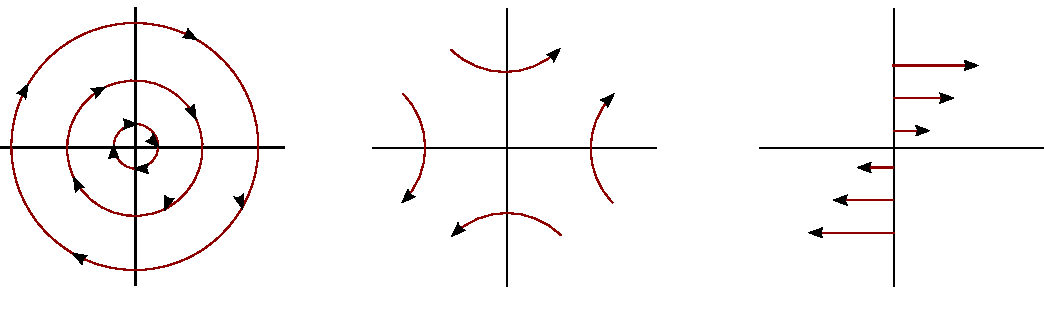
\includegraphics[width=1.2\textwidth]{figs/shear_decomposition}}
\begin{lpic}{figs/shear_decomposition(10cm,)}
   \lbl[b]{25,0;\vphantom{Hq}Rotation}
   \lbl[b]{85,0;\vphantom{Hq}stretching}
   \lbl[b]{152,0;\vphantom{Hq}shear}
   \lbl[c]{55,30;$+$}
   \lbl[c]{120,30;$=$}
   \lbl[b]{55,0;\vphantom{Hq}$+$}
   \lbl[b]{120,0;\vphantom{Hq}$=$}
\end{lpic}  
\caption{\label{fig:shear_decomposition} Decomposition of the simple shear flow into rotation and strain.}%
\end{figure}


\section{The Jeffery equation and its solutions}\seclab{jefferyequation}

The main result of \citet{jeffery1922} is the hydrodynamic torque $\ve T$ on a general ellipsoid rotating in a viscous shear flow (his Eq.~(36)). In other words, he computed the elements of the resistance tensors in \Eqnref{resistanceformulation}. Some elements were known to Jeffery from earlier work by \citet{oberbeck1876} and \citet{edwardes1893}. However, Jeffery completed arguably the hardest part of the calculation, and has received the most credit for this work.

The viscous torque is calculated neglecting the effects of fluid inertia, $\Reys=0$. To be consistent (see \Secref{stokesnumber}) we will also neglect the effects of particle inertia, $\st=0$. This is the overdamped limit where the equation of motion is determined by a static force and torque balance. Jeffery found the angular velocity of the particle by solving $\ve T=0$. Here I give the result in my notation, the details are available in \Appref{triaxial_equation}.

We represent the shape and orientation of an ellipsoid by the lengths $(a_1, a_2, a_3)$ and directions $(\ve n_1, \ve n_2, \ve n_3)$ of the three half-axes. Then $\ve n_1$ gives the direction of the axis with length $a_1$, and so on. The angular velocity depends on the flow gradients, the particle orientation and the aspect ratios of the particle. 
\begin{align}
	\ve \omega &= \ve \Omega
	 + K\left(\ve n_2\transpose \ma S\ve n_3\right)\ve n_1
	 - \Lambda\left(\ve n_3\transpose \ma S\ve n_1\right)\ve n_2
	  + \frac{K- \Lambda}{K \Lambda - 1}\left(\ve n_1\transpose \ma S\ve n_2\right)\ve n_3,\eqnlab{triaxialomega}
\end{align}
where
\begin{align}
	K=\frac{\kappa^2-1}{\kappa^2+1}, \qquad \Lambda=\frac{\lambda^2-1}{\lambda^2+1},\qquad \lambda=a_1/a_3, \qquad \kappa=a_2/a_3\,.
\end{align}
Here $\ve \Omega$ and $\ma S$ are the flow rotation and strain as defined in \Secref{fluidflows}. The coefficients $\Lambda$ and $K$ are the \emph{shape parameters}, and for an ellipsoid $-1 < \Lambda, K < 1$. A sphere is described by $\Lambda=K=0$. If either $\Lambda$ or $K$ is zero, the particle is an axisymmetric spheroid. \Eqnref{triaxialomega} is valid for most particles with the same mirror symmetries as an ellipsoid, with a suitable redefinition of $\Lambda$ and $K$ \cite{bretherton1962,happel1965,kim1991}. More precisely, there are other particle shapes described by resistance tensors of the same \emph{form}, but different numerical values of the elements.

We rename $\ve n = \ve n_1$ and $\ve p=\ve n_2$, and compute their equation of motion by $\dot{\ve n}_i=\ve \omega \cross \ve n_i$ (details in \Appref{triaxial_equation}):
\begin{align}
	\dot{\ve n}	&= \ma O \ve n 
	+ \Lambda\left(
	\ma S \ve n - (\ve n \transpose \ma S \ve n) \ve n
	\right)
    + \frac{K(1- \Lambda^2)}{K \Lambda - 1}\left(\ve n\transpose \ma S\ve p\right)\ve p,  \nn\\
\dot{\ve p}	&=    \ma O \ve p
	 + K\left(
\ma S \ve p  - (\ve p \transpose \ma S \ve p) \ve p
	 \right)
	  + \frac{\Lambda(1-K^2)}{K \Lambda - 1}\left(\ve n\transpose \ma S\ve p\right)\ve n\,. \eqnlab{np}
\end{align}
\Eqnref{np} is the Jeffery equation of motion for a the axes of an triaxial ellipsoid. Recall that $\ma O \ve n=\ve \Omega \cross \ve n$. The motion of the third axis is fully determined by $\ve n_3 = \ve n \cross \ve p$. The equations are symmetric under the simultaneous exchange of $\Lambda\leftrightarrow K$ and $\ve n\leftrightarrow\ve p$, because the new equations describe the same physical situation with the axes permuted.

In the following Sections we will study the solutions to \Eqnref{np} in some detail. But it is helpful to first inspect the meaning of the different terms in the equation of motion:

The first term means that the particle is rotated by the local flow vorticity, and that this rotation is independent of the particle shape.

The second term means that the local rate-of-strain attracts the particle axis to the strongest eigendirection of $\ma S$. The strength of the attraction is affected by the particle shape. The more elongated an axis is, the stronger the attraction becomes. The non-linear part $- (\ve n \transpose \ma S \ve n) \ve n$ simply preserves the unit magnitude of the vector $\ve n$, and it has no physical meaning. This fact is explained in detail in \Secref{jeffaxisymmetric}. 

The third and last term couples the motion of $\ve n$ and $\ve p$. This is because the local rate-of-strain will try to align all elongated axes. But since the particle is a rigid body, this is not possible. Instead there is competition, and the outcome depends on the relative elongation of the axes. If the particle is axisymmetric, say $K=0$, there is only one elongated axis and therefore no competition. This case is described in detail in \Secref{jeffaxisymmetric}. The general case of a triaxial ellipsoid in a simple shear flow is discussed in \Secref{jefftriaxial}.

\subsection{Axisymmetric particles}\seclab{jeffaxisymmetric}

In this section we consider axisymmetric particles: particles which are rotationally symmetric around an axis of symmetry. For such particles the shape factor $K=0$, and \Eqnref{np} reduces to
\begin{align}
	\dot{\ve n}	&= \ma O \ve n 
	+ \Lambda\left(
	\ma S \ve n - (\ve n \transpose \ma S \ve n) \ve n
	\right),  \eqnlab{npaxin}\\
\dot{\ve p}	&=    \ma O \ve p
	  -\Lambda\left(\ve n\transpose \ma S\ve p\right)\ve n\,. \eqnlab{npaxip}
\end{align}

\begin{figure}
\centering
\begin{overpic}[unit=1mm]{figs/naxidef.pdf}
\put(0,55){\parbox[t][20mm][t]{40mm}{\centering Oblate\\$\Lambda < 0$}}
\put(50,55){\parbox[t][20mm][t]{40mm}{\centering Prolate\\$\Lambda > 0$}}
\put(21,39){$\ve n$}
\put(95,47){$\ve n$}
\end{overpic}
\caption{\label{fig:naxidef} Illustration of axisymmetric particles and the definition of the vector $\ve n$. \emph{Left}: Oblate, disk-shaped particle. \emph{Right}: Prolate, rod-shaped particle.}%
\end{figure}


The vector $\ve n$ describes the direction of the symmetry axis of the particle, see \Figref{naxidef}. The vector $\ve p$ describes the rotation around the symmetry axis. The equations for $\ve n$ and $\ve p$ are decoupled: we may first solve \Eqnref{npaxin} for $\ve n(t)$, then \Eqnref{npaxip} is a linear equation for $\ve p(t)$. In this Section we will neglect the dynamics of $\ve p$, it is discussed in \Secref{jefftriaxial}. 

\Eqnref{npaxin} is a non-linear vector equation, and as such it is seemingly hard to solve. However, the non-linearity is only apparent: it is due to the geometric constraint that $\ve n$ is a unit vector. The underlying dynamics is in fact linear. I will now explain two ways to understand this fact.

The vorticity $\ma O$ rotates $\ve n$, and the strain $\ma S$ aligns and stretches $\ve n$ towards its strongest eigendirection. The non-linear term $\ve n \ve n\transpose \ma S \ve n$ is simply the stretching component of the strain, which is subtracted in order to prevent elongation of $\ve n$. Bretherton (Sec.~6 in Ref.~\citenum{bretherton1962}) realised that we may instead model the orientation of the particle with any vector $\ve q$ which obeys the same linear terms, but without compensating for any elongation:
\begin{align}
	\dot{\ve q} = \left(\ma O + \Lambda \ma S\right) \ve q.\eqnlab{jefferyq}
\end{align}
Owing to the common linear terms in \Eqnref{npaxin} and \Eqnref{jefferyq}, the vector $\ve q$ will have the same angular dynamics as $\ve n$. In addition, $\ve q$ may be stretched and compressed by the strain $\ma S$. But since we are only interested in the angular degrees of freedom, we can at any instant recover $\ve n$ by normalising $\ve q$ to unit length. Thus, the general solution of the Jeffery equation is given by solving \Eqnref{jefferyq} for $\ve q(t)$, then the solution to \Eqnref{npaxin} is given by normalising $\ve q(t)$ to unit length:
\begin{align}
	\ve n(t) &= \frac{\ve q(t)}{|\ve q(t)|}.\eqnlab{jefferysolution0}
\end{align}

Another, more mathematical, way of understanding how the linear companion equation \eqnref{jefferyq} arises is the following. Like above, we choose to represent the particle orientation by a vector $\ve q$ which is parallel to $\ve n$. Define $\ve q = \alpha(t)\ve n$, with $\alpha(t)$ an arbitrary function of time. We know from this definition that we may always recover $\ve n$ by normalising $\ve q$ to unit length. Now, we can calculate the equation of motion for $\ve q$:
\begin{align}
	\diff{\ve q}{t} &= \diff{}{t}\left(\alpha \ve n\right) \nn \\
	&= \dot \alpha \ve n + \alpha \dot{\ve n} \nn\\
	&= \dot \alpha \ve n + \alpha \left(\ma O \ve n + \Lambda \left(\ma S \ve n - \ve n \ve n \transpose \ma S \ve n\right)\right). \eqnlab{jefferyderivation1}
\end{align}
But $\alpha(t)$ is an arbitrary function which we may choose. In particular we can choose $\alpha(t)$ to be a function satisfying
\begin{align}
	\dot \alpha &= \alpha \Lambda \ve n\transpose \ma S \ve n.
\end{align}
By inserting this choice of $\alpha(t)$ into \Eqnref{jefferyderivation1}, we again arrive at \Eqnref{jefferyq}.

We will now consider the solutions of Jeffery's equation in a time-independent linear flow. This case includes for example the simple shear flow. It is also a useful model when the flow changes only slowly in time, compared to the time it takes for the gradients to affect the particle orientation. First, I will describe the possible solutions of \Eqnref{npaxin} in linear flows. Second, I will discuss the solutions of Jeffery's equation in a simple shear flow. These solutions are called the Jeffery orbits, and they play an important role in Papers~A-F.

When $\ma O$ and $\ma S$ are time-independent the linear companion equation \eqnref{jefferyq} is solved by the matrix exponential:
\begin{align}
		\ve q(t) = e^{(\ma O + \Lambda \ma S)t}\ve q(0).
\end{align}
This solution implies that the long-time dynamics of $\ve q$, and therefore $\ve n$, is determined by the eigenvalues and eigenvectors of the matrix $\ma B = \ma O + \Lambda\ma S$. For an incompressible flow $\tr\ma B=0$, because $\tr\ma A=0$. In three spatial dimensions, the three eigenvalues of $\ma B$ must sum to zero. Thus, as noted by Bretherton \cite{bretherton1962}, there are four distinct possibilities for the eigensystem of $\ma B$:
\begin{enumerate}
	\item Three real eigenvalues, then
	\item[] $\ve q$ will align with the eigenvector corresponding to the largest eigenvalue.
	\item One real eigenvalue $a>0$, and a complex pair $-a/2 \pm i\omega$, then
	\item[] $\ve q$ will spiral into alignment with the eigenvector corresponding to the real eigenvalue.
	\item One real eigenvalue $a<0$, and a complex pair $-a/2 \pm i\omega$, then
	\item[] $\ve q$ will spiral out towards infinity in the plane that contains the origin and is spanned by the real and imaginary parts of the complex eigenvector.
	\item One real eigenvalue $a=0$, and an imaginary pair $\pm i\omega$, then
	\item[] $\ve q$ rotates indefinitely in a closed elliptic orbit in a plane that contains the initial condition and is spanned by the real and imaginary parts of the complex eigenvector.
\end{enumerate}
\begin{figure}
\centering
\makebox[\textwidth]{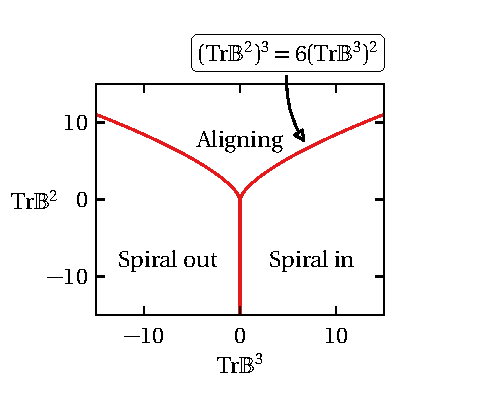
\includegraphics{figs/bmap}}
\caption{\label{fig:bmap}  Map of the three possible types of particle motion, as determined by the eigensystem of $\ma B=\ma O + \Lambda \ma S$. On the red line between ``Spiral out'' and ``Spiral in'' the motion is on a closed orbit.}%
\end{figure}
The characteristic equation for the eigenvalues $b$ of a $3\times3$-matrix $\ma B$ is
\begin{align}
	-b^3 + b^2\tr \ma B  + \frac{b}{2}\left(\tr \ma B^2-(\tr \ma B)^2\right)+\det\ma B = 0.
\end{align}
But for a traceless matrix $\tr \ma B=0$ and $\det \ma B = \tr\ma B^3/3$, because
\begin{align}
	\tr \ma B &= b_1 + b_2 + b_3 = 0 \implies b_3 = -(b_1 + b_2),\\
	\intertext{therefore}
	\tr \ma B^3 &= b_1^3 + b_2^3 + b_3^3 = -3(b_1^2b_2 + b_1b_2^2),\\
	\det \ma B &= b_1b_2b_3 = -(b_1^2b_2 + b_1b_2^2).
\end{align}
Thus the characteristic equation simplifies to
\begin{align}
	-b^3 + \frac{b}{2}\tr \ma B^2 +\frac{1}{3}\tr\ma B^3 = 0. \eqnlab{bcharacteristic}
\end{align}
It is possible to solve \Eqnref{bcharacteristic} exactly for the eigenvalues, but the important observation is that they are determined by only two parameters: $\tr \ma B^2$ and $\tr\ma B^3$. In Fig.~\ref{fig:bmap} I illustrate how the three cases outlined above correspond to different values of $\tr \ma B^2$ and $\tr\ma B^3$. The boundary curve of the region of three real eigenvalues is where the discriminant $\Delta$ of the characteristic equation is zero:
\begin{align}
 	\Delta = \left(\tr \ma B^2\right)^3 - 6\left(\tr \ma B^3\right)^2 = 0.
 \end{align} 
In the region where there is a pair of complex eigenvalues, the two cases of spiral in or out are separated by $\tr \ma B^3=0$. For any given flow gradient, changing the particle from rod-like to disk-shaped (or vice versa) transforms $\tr \ma B^3\to-\tr\ma B^3$ and therefore change the qualitative dynamics from aligning to rotating (or vice versa). This transformation may be understood because
\begin{align}
	\tr \ma B^3 = 3\Lambda \tr \ma O\ma O \ma S + \Lambda^3 \tr \ma S\ma S \ma S.
\end{align}
The other combinations of $\ma S$ and $\ma O$ which could be expected to contribute, such as $\tr \ma O\ma O \ma O$, vanish identically because of symmetries of $\ma O$ and $\ma S$. As explained above, changing a particle from rod-like to disk-shaped implies a change of sign of the shape factor $\Lambda$. We discussed the implications of this observation for the tumbling of particles in turbulent and random flows, in an earlier paper \cite{gustavsson2014}.

\subsubsection{The Jeffery Orbits}\seclab{jefferyorbits}

The remainder of this section concerns the case of simple shear flow. This case is characterised by $\tr \ma B^3=0$ and $\tr \ma B^2<0$. The simple shear has a special position among flows, and we understand the significance of the condition $\tr\ma B^3=0$ from the above discussion: First, a change of particle shape does not change the qualitative dynamics. Both disk-shaped particles and rod-like particles rotate in a shear flow. Second, $\ma B$ has a zero eigenvalue, as seen from the characteristic equation \eqnref{bcharacteristic}. The zero eigenvalue is important, because it implies that the particle dynamics never forgets its initial condition. The eigenvector of the zero eigenvalue is the vorticity direction\footnote{See Fig.~\ref{fig:coordinates} and Sec.~\ref{sec:shearflow} for the definition of the coordinate system and the terminology of its directions in a simple shear flow.}, thus the component of $\ve q$ in the vorticity direction is constant in a shear flow. The other two eigenvalues form an imaginary pair, resulting in a periodic rotation of $\ve q$.

In summary, the dynamics of $\ve q$ in a simple shear flow is a periodic rotation in a plane. The plane is normal to the vorticity direction, and determined by the initial condition of $\ve q$.

\begin{figure}
	  \makebox[\textwidth]{%
        \begin{subfigure}[b]{0.5\textwidth}
                \centering
                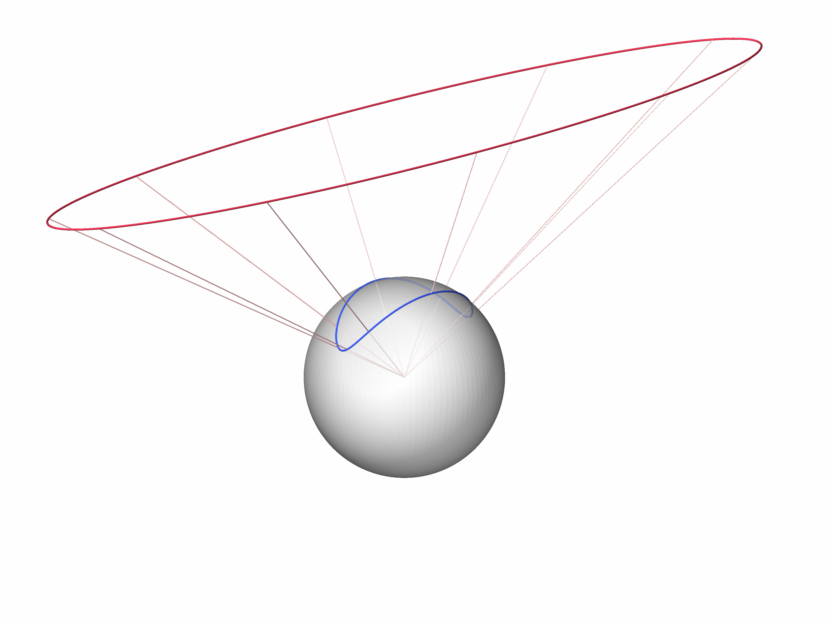
\includegraphics[width=\textwidth]{figs/projection_orbit1.png}
                \caption{}
                \label{fig:projection_orbit1}
        \end{subfigure}%
        \begin{subfigure}[b]{0.5\textwidth}
                \centering
                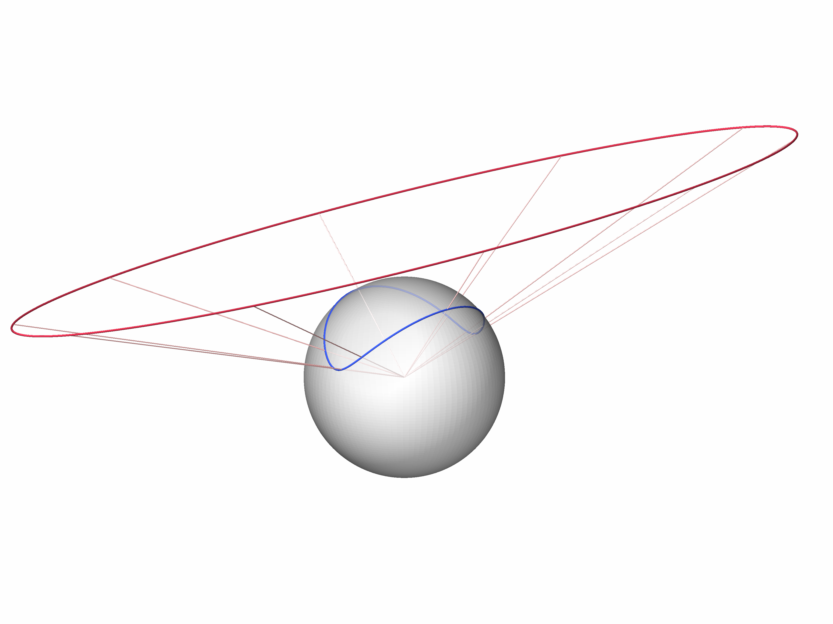
\includegraphics[width=\textwidth]{figs/projection_orbit2.png}
                \caption{}
                \label{fig:projection_orbit2}
        \end{subfigure}
        }
        \makebox[\textwidth]{%
        \begin{subfigure}[b]{0.5\textwidth}
                \centering
                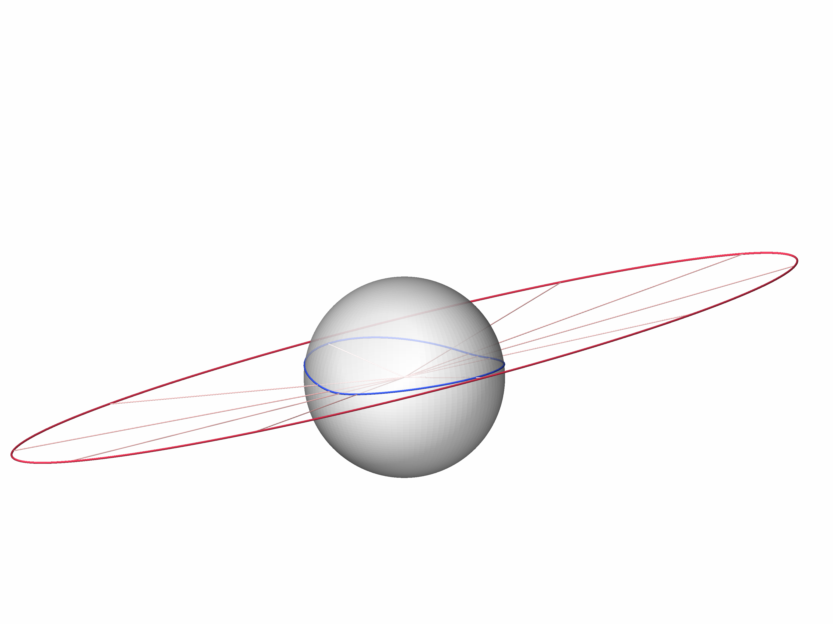
\includegraphics[width=\textwidth]{figs/projection_orbit3.png}
                \caption{}
                \label{fig:projection_orbit3}
        \end{subfigure}
        \begin{subfigure}[b]{0.5\textwidth}
                \centering
                %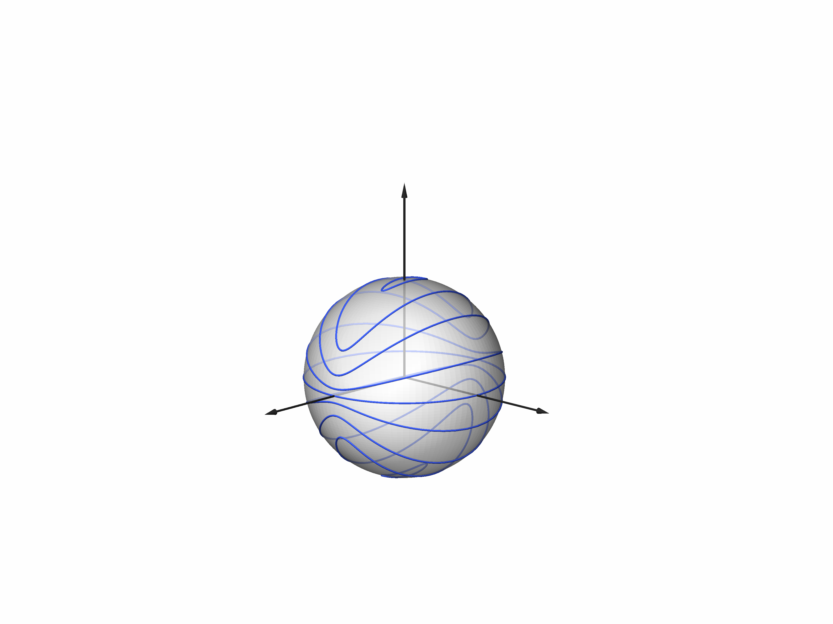
\includegraphics[width=\textwidth]{figs/projection_orbit4.png}
				\begin{lpic}{figs/projection_orbit4(7cm,)}
				   \lbl[tl]{60,55;$\hat{\ve x}$}
				   \lbl[tl]{150,55;$\hat{\ve y}$}
				   \lbl[tl]{105,130;$\hat{\ve z}$}
				\end{lpic}
                \caption{}
                \label{fig:projection_orbit4}
        \end{subfigure}        
	  }%
    \caption{\textbf{(a-c)} Illustrations of how the trajectories $\ve q(t)$ (red) produces the Jeffery orbits $\ve n(t)$ (blue) upon projection onto the unit sphere. \textbf{(d)} Sample of resulting Jeffery orbits with coordinate system. All trajectories correspond to a particle of aspect ratio $\lambda=5$ in a simple shear flow.}\label{fig:projection_orbits}
\end{figure}

When the trajectories $\ve q(t)$ are projected onto the unit sphere, the result $\ve n(t)$ are the Jeffery orbits. I visualise this in Fig.~\ref{fig:projection_orbits} where the trajectories $\ve q(t)$ and $\ve n(t)$ are shown for three different initial conditions.

The orbits on the north and south hemispheres are the same, because of the particle inversion symmetry: changing $\ve n \to -\ve n$ implies $\dot{\ve n} \to - \dot{\ve n}$. The orbits are also symmetric under a 180 degree rotation around the vorticity, becuse the shear flow is. These two symmetries together enforce that no orbit may cross the equator of the sphere. The Jeffery orbit which is exactly on the equator of the sphere is called the \emph{tumbling orbit}, because the vector $\ve n$ tumbles in the flow-shear plane. The orbit at a pole of the sphere, where $\ve n$ is aligned with the vorticity direction, is called the \emph{log-rolling} orbit. The name refers to the motion of a rod which rolls around its axis of symmetry, but the name is used for both prolate and oblate particles. Log-rolling for an oblate particle means that it spins like a frisbee. These particular orbits are depicted in \Figref{tumbling_lr}.

The solutions to Jeffery's equation in a simple shear flow are degenerate: the orientational trajectory depends on the initial condition indefinitely. The degeneracy is a result of the assumptions made in the course deriving the Jeffery orbits. In this thesis we encounter two possible mechanisms to break this degeneracy.

First, there may be inertial effects. The Jeffery equation neglects the effects of both fluid and particle inertia. In fact, Jeffery suggested that inertia should dissolve the degeneracy and lead to a determinate prediction. My work in the Papers~A-D resolves this question. Although Jeffery was right in principle, it did not turn out exactly like he envisaged it. This is described in detail in \Secref{effective} in Part II.

Second, there may be Brownian noise. The idea is that thermal fluctuations kick the particle out of one Jeffery orbit and into another. After some time, the initial condition is forgotten and the state of the particle is described by an orientational probability distribution. This line of work formed the basis of the theories describing the rheology of dilute particle suspensions.

One might expect that the degeneracy of the Jeffery orbits could be broken by a particle which is not perfectly axisymmetric. This is not the case. However, the dynamics are much more intricate. This is the topic of \Secref{jefftriaxial}.


\begin{figure}
\centering
\begin{overpic}[unit=1mm,scale=0.5]{figs/coords_prolate_tumbling.pdf}
\put(0,70){\textbf{\small(a)}}
\put(-5,2){$\hat{\ve x}$}
\put(101,12){$\hat{\ve y}$}
\put(54,87){$\hat{\ve z}$}
\end{overpic}\qquad\qquad
\begin{overpic}[unit=1mm,scale=0.5]{figs/coords_oblate_tumbling.pdf}
\put(0,70){\textbf{\small(b)}}
\put(-5,2){$\hat{\ve x}$}
\put(101,12){$\hat{\ve y}$}
\put(54,87){$\hat{\ve z}$}
\end{overpic}\\\vspace{5mm}
\begin{overpic}[unit=1mm,scale=0.5]{figs/coords_prolate_lr.pdf}
\put(0,70){\textbf{\small(c)}}
\put(-5,2){$\hat{\ve x}$}
\put(101,12){$\hat{\ve y}$}
\put(54,87){$\hat{\ve z}$}
\end{overpic}\qquad\qquad
\begin{overpic}[unit=1mm,scale=0.5]{figs/coords_oblate_lr.pdf}
\put(0,70){\textbf{\small(d)}}
\put(-5,2){$\hat{\ve x}$}
\put(101,12){$\hat{\ve y}$}
\put(54,87){$\hat{\ve z}$}
\end{overpic}\\\vspace{5mm}
\caption{\figlab{tumbling_lr} Illustration of the tumbling and log-rolling orbits it a simple shear flow. \textbf{(a)} prolate tumbling, \textbf{(b)} oblate tumbling, \textbf{(c)} prolate log-rolling, \textbf{(d)} oblate log-rolling.}%
\end{figure}


\subsection{Non-axisymmetric particles}\seclab{jefftriaxial}

In this Section I describe the solutions to the Jeffery equation \eqnref{np} for a triaxial particle in a simple shear flow. It turns out that a triaxial particle also tumbles, but in a much more complicated fashion than the Jeffery orbits for an axisymmetric particle \cite{gierszewski1978,hinch1979,yarin1997}. In general no closed form solutions are known, therefore we rely on numerical solutions in this section.

A rotation in three dimensions has three degrees of freedom, and can be represented in different ways. In general it is complicated to represent rotations, because the space of rotations $SO(3)$ does not simply map to $\ma R^3$. Fortunately the tumbling of a triaxial particle shares one property with the Jeffery orbits: the vector $\ve n$ monotonically rotates around the vorticity. This fact was proven by \citet{hinch1979}. They expressed \Eqnref{np} in Euler angle coordinates, such that $(\varphi, \theta)$ are spherical coordinates for $\ve n$ (\Figref{coordinates}), and $\psi$ is the angle of rotation around $\ve n$. Then $\dot\varphi < 0$ for all values of $\Lambda$ and $K$. It follows that it is sufficient to observe the trajectories the as they pass through a plane in phase space, as depicted in \Figref{sos}. The monotonic rotation guarantees that all trajectories hit the surface-of-section, over and over again.

\begin{figure}
\centering
\begin{overpic}[unit=1mm,width=10cm]{figs/sos.png}
\put(70,84){$\varphi = \pi/2+2n\pi$}
\put(75,5){$\big[\varphi(t),\theta(t),\psi(t)\big]$}
\end{overpic}
\caption{\label{fig:sos} Illustration of the surface-of-section $\varphi=\pi/2+2n\pi$. The trajectory (in red) starts at a point in the surface-of-section, makes one revolution of $\varphi $in phase-space, and returns to another point on the same curve in the surface-of-section.}%
\end{figure}

We follow \citet{hinch1979} and choose the surface-of-section $\varphi = \pi/2+2n\pi$. This corresponds to $n_x=0, n_y > 0$. We solve \Eqnref{np} numerically for many different initial conditions. Every time a trajectory passes through the surface-of-section we plot a point at the corresponding value of $n_z=\cos \theta$ and $\psi$. Four examples for $\lambda=5$ and increasing values of $\kappa$ are shown in Figs.~\ref{fig:poincare1o00}-\ref{fig:poincare2o00}.

\Figref{poincare1o00} shows the surface-of-section for an axisymmetric particle. The horizontal lines are the Jeffery orbits of an axisymmetric particle. Every time a trajectory reaches the surface-of-section, the value of $n_z$ is the same, because of the perodicity of the Jeffery orbit. However, it turns out that the value of $\psi$ is in general not periodic. This means that the vector $\ve p$ does not, in general, make one revolution around $\ve n$ for every Jeffery orbit. The strict periodicity of the Jeffery orbits really only apply to the motion of the symmetry axis. This detail has no physical implications for the motion. But if we were to paint a pattern on a particle, and observe the motion experimentally, this aperiodicity would be apparent.

For the trajectory of a nearly axisymmetric particle neither $n_z$, nor $\psi$ is constant. The structure of trajectories on the surface-of-section is more complicated, with closed ellipses near $n_z\approx 0$, and curved lines towards $n_z\approx\pm 1$, shown in \Figref{poincare1o10}.
However, a trajectory is always confined to the curve on which it started. In this sense the orientational dynamics of a triaxial particle is degenerate, just like the Jeffery orbits for an axisymmetric particle. No orbit is physically preferred over any other, but the dynamics are determined by the initial condition.

When we consider a significantly non-axisymmetric particle, the trajectories on the surface-of-section look very different, like in \Figref{poincare1o30} and \Figref{poincare2o00}. Many initial conditions lead to deterministic chaos, which shows up as areas full of gray dots without apparent structure. A trajectory starting in this chaotic layer can go anywhere else inside it.

\begin{figure}
\centering
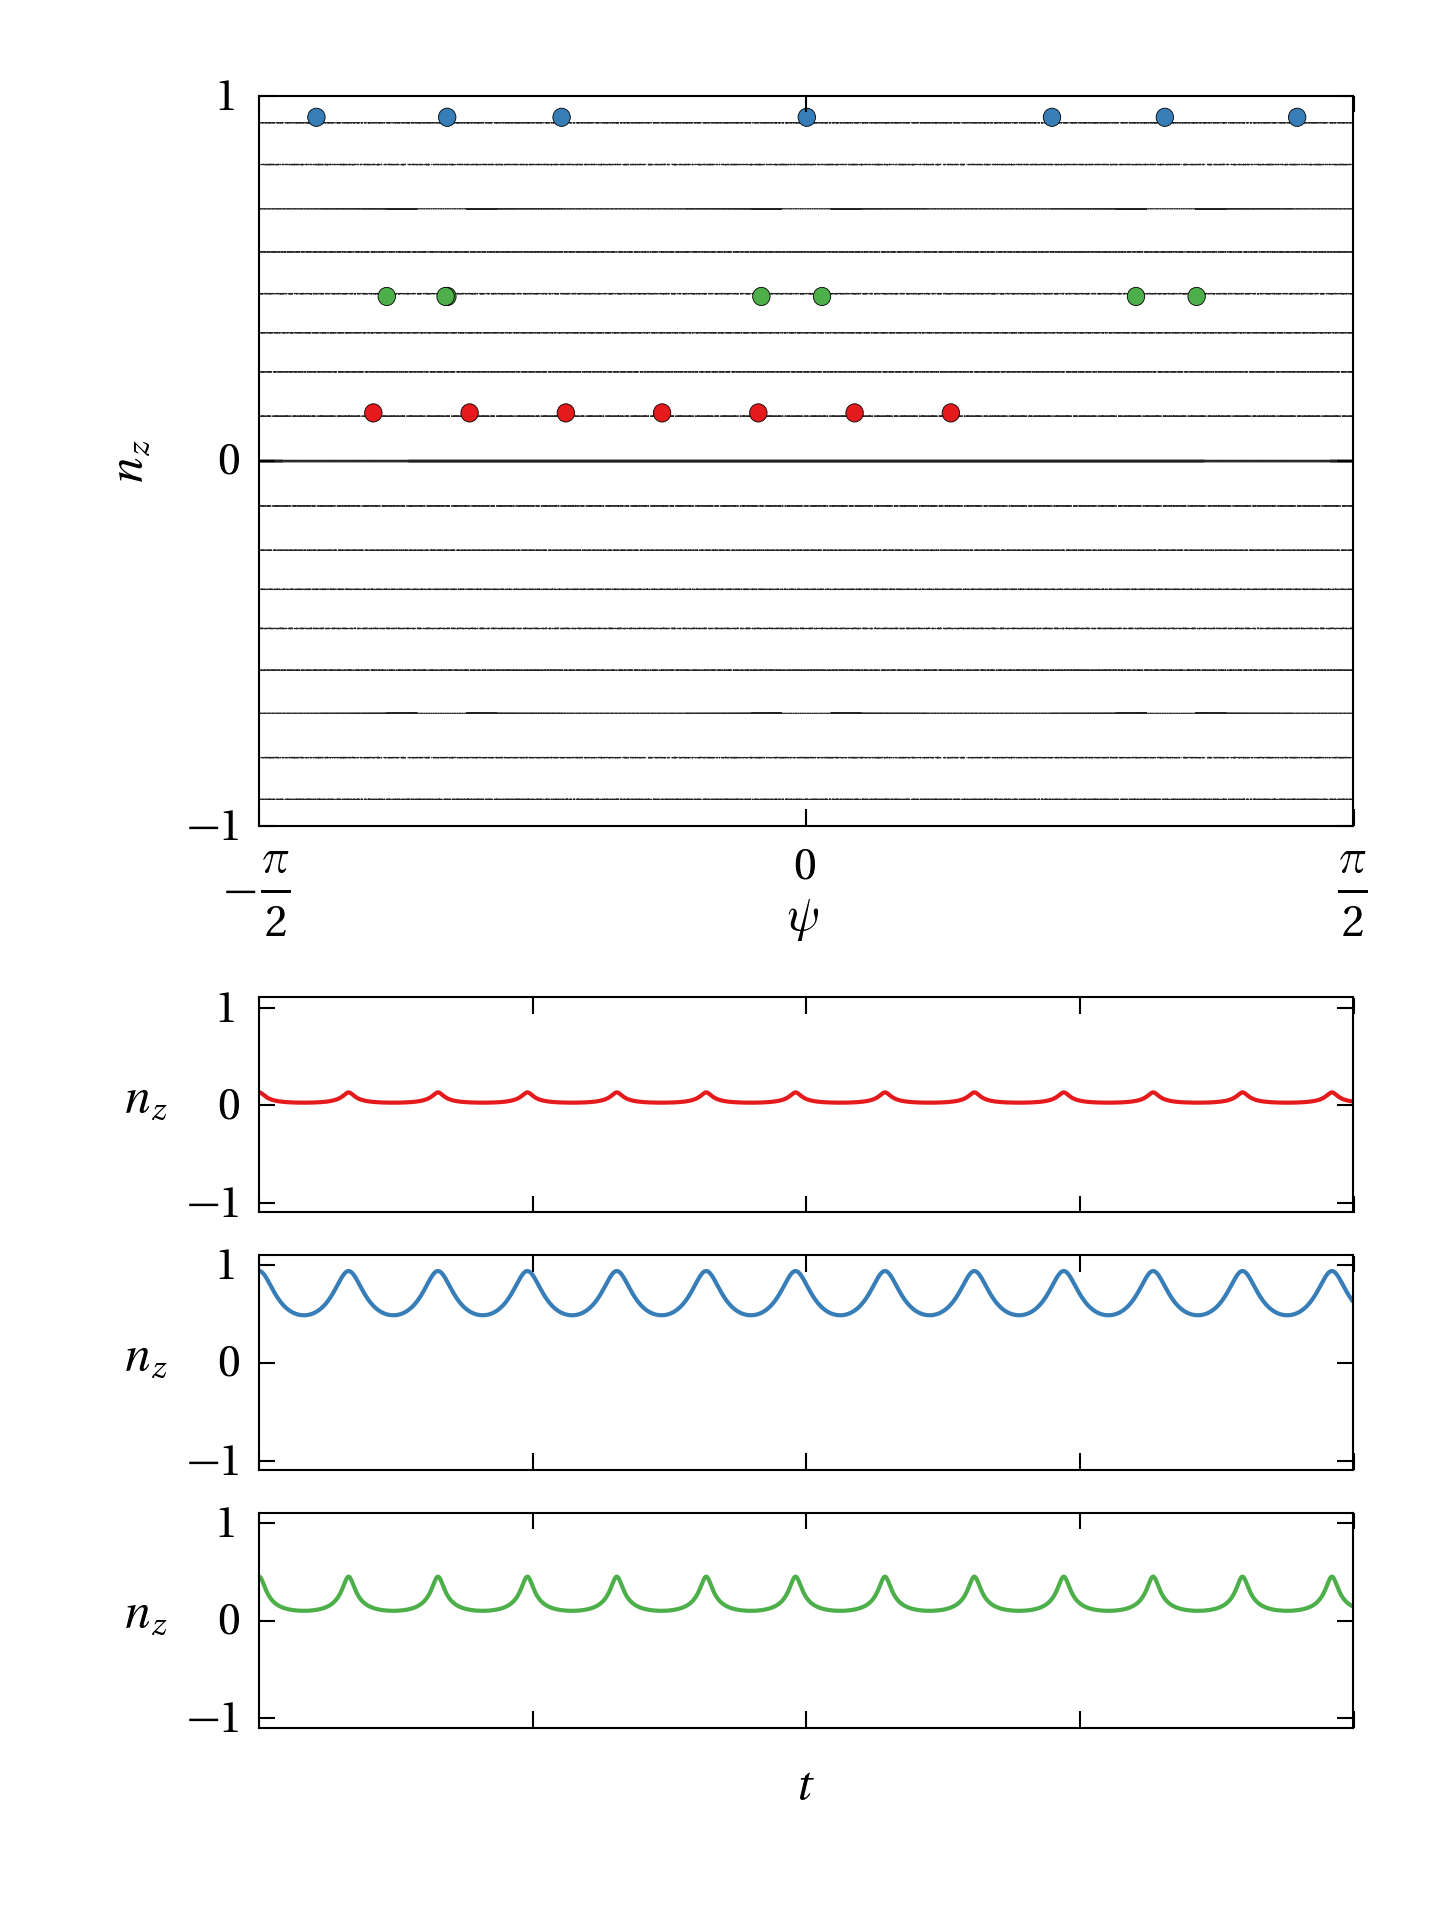
\includegraphics[width=12cm]{figs/poincare1o00.png}%
\caption{\label{fig:poincare1o00} Top: Poincar\'e surface-of-section of an axisymmetric particle with aspect ratios $\lambda=5$, $\kappa=1$. Bottom: Examples of what $n_z(t)$ looks like, given the trajectory indicated by the color coded markers on the surface-of-section. 
}
\end{figure}
\begin{figure}
\centering
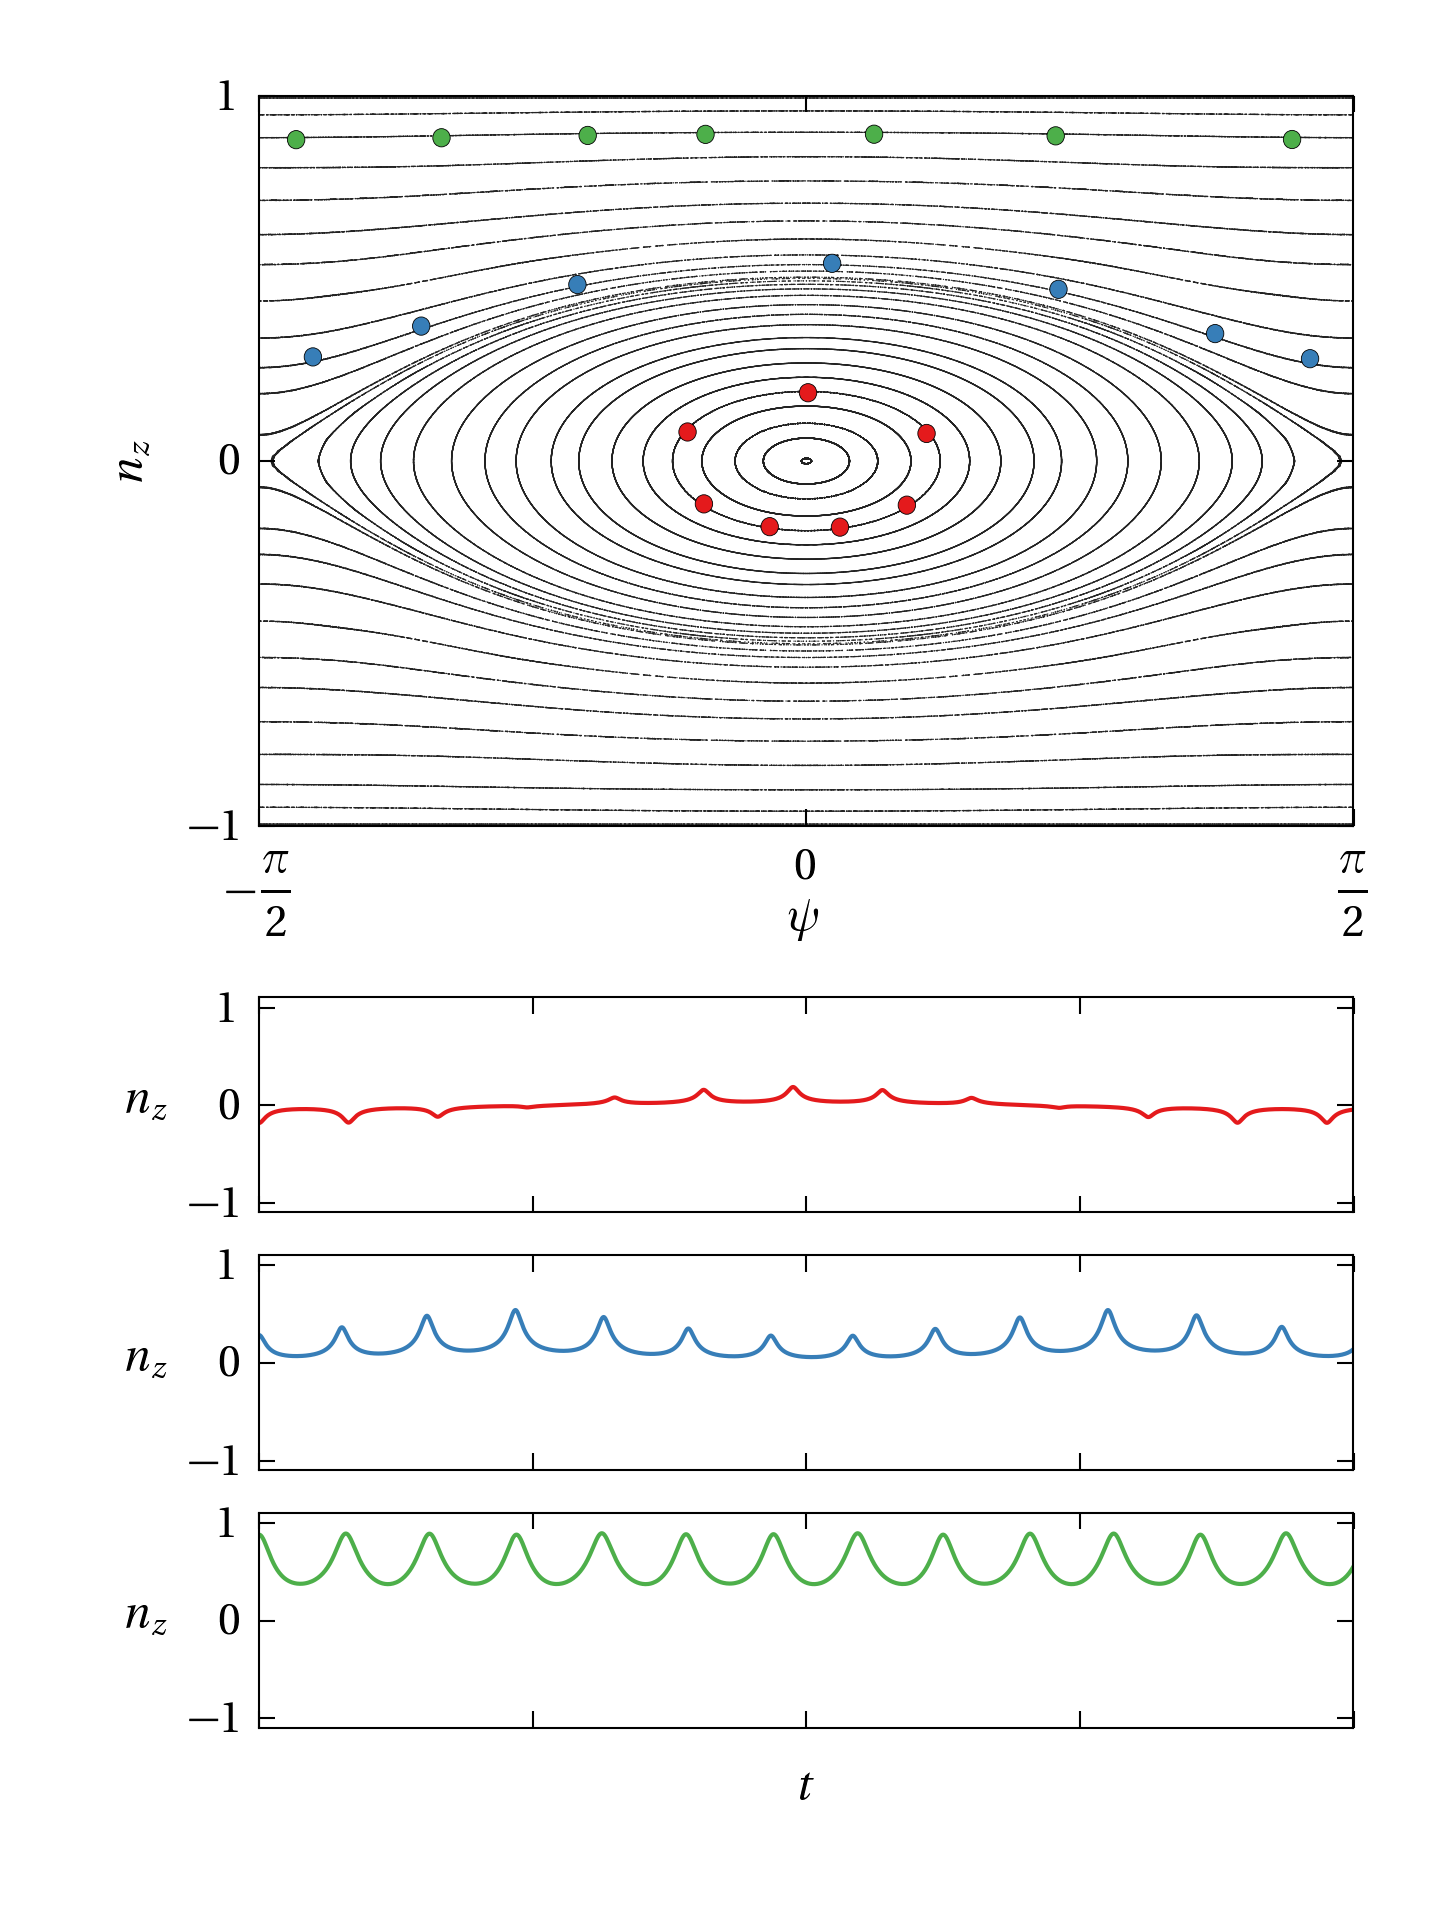
\includegraphics[width=12cm]{figs/poincare1o10.png}%
\caption{\label{fig:poincare1o10} Top: Poincar\'e surface-of-section of an asymmetric particle with aspect ratios $\lambda=5$, $\kappa=1.1$. Bottom: Examples of what $n_z(t)$ looks like, given the trajectory indicated by the color coded markers on the surface-of-section. 
}
\end{figure}
\begin{figure}
\centering
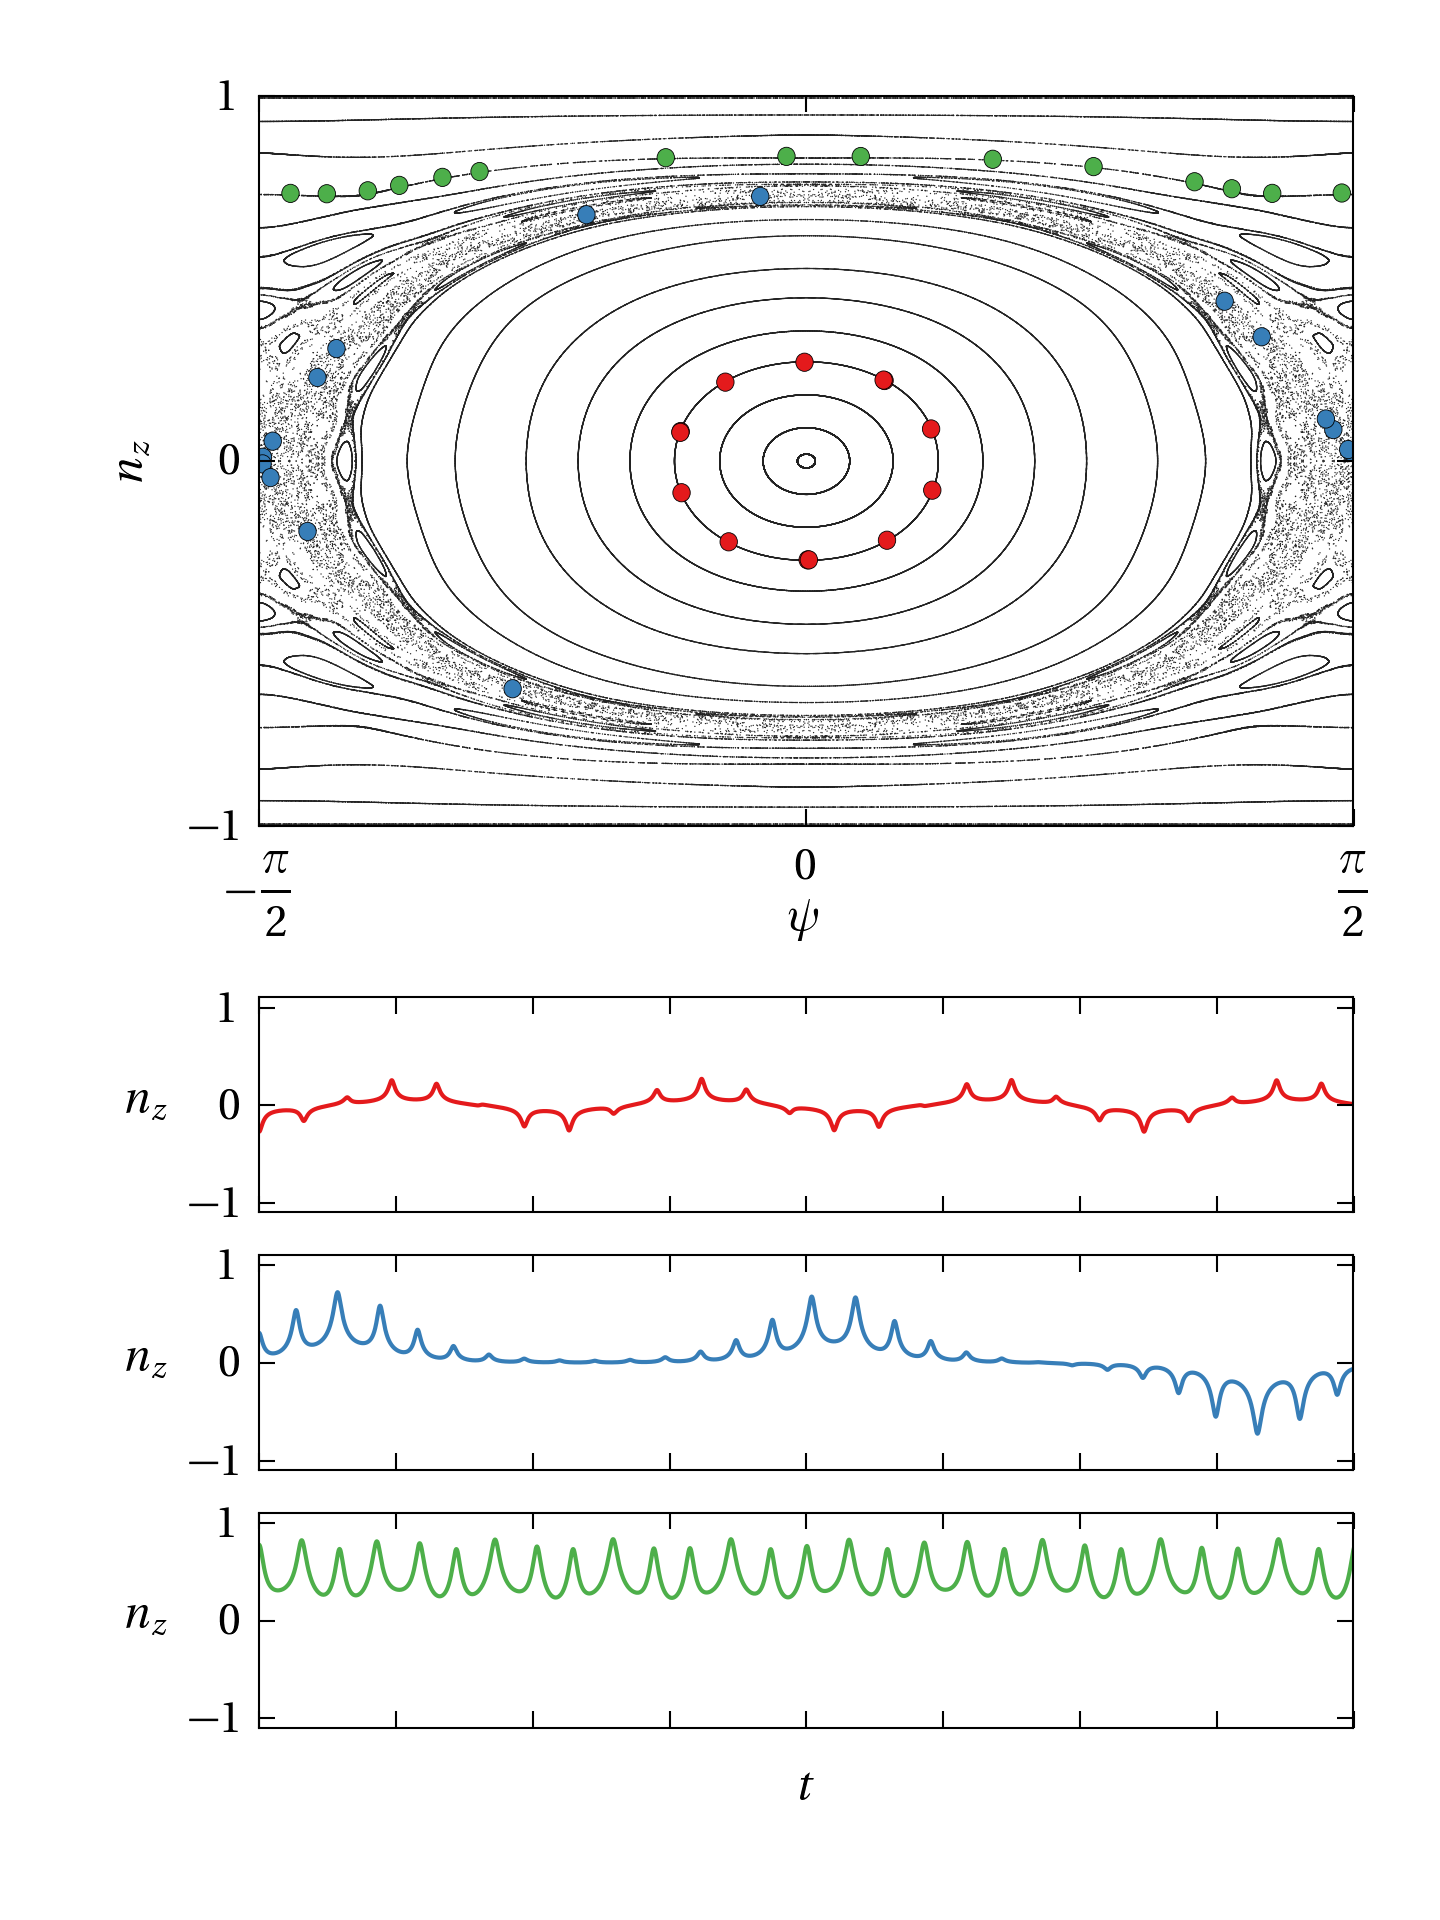
\includegraphics[width=12cm]{figs/poincare1o30.png}%
\caption{\label{fig:poincare1o30} Top: Poincar\'e surface-of-section of an axisymmetric particle with aspect ratios $\lambda=5$, $\kappa=1.3$. Bottom: Examples of what $n_z(t)$ looks like, given the trajectory indicated by the color coded markers on the surface-of-section. 
}
\end{figure}
\begin{figure}
\centering
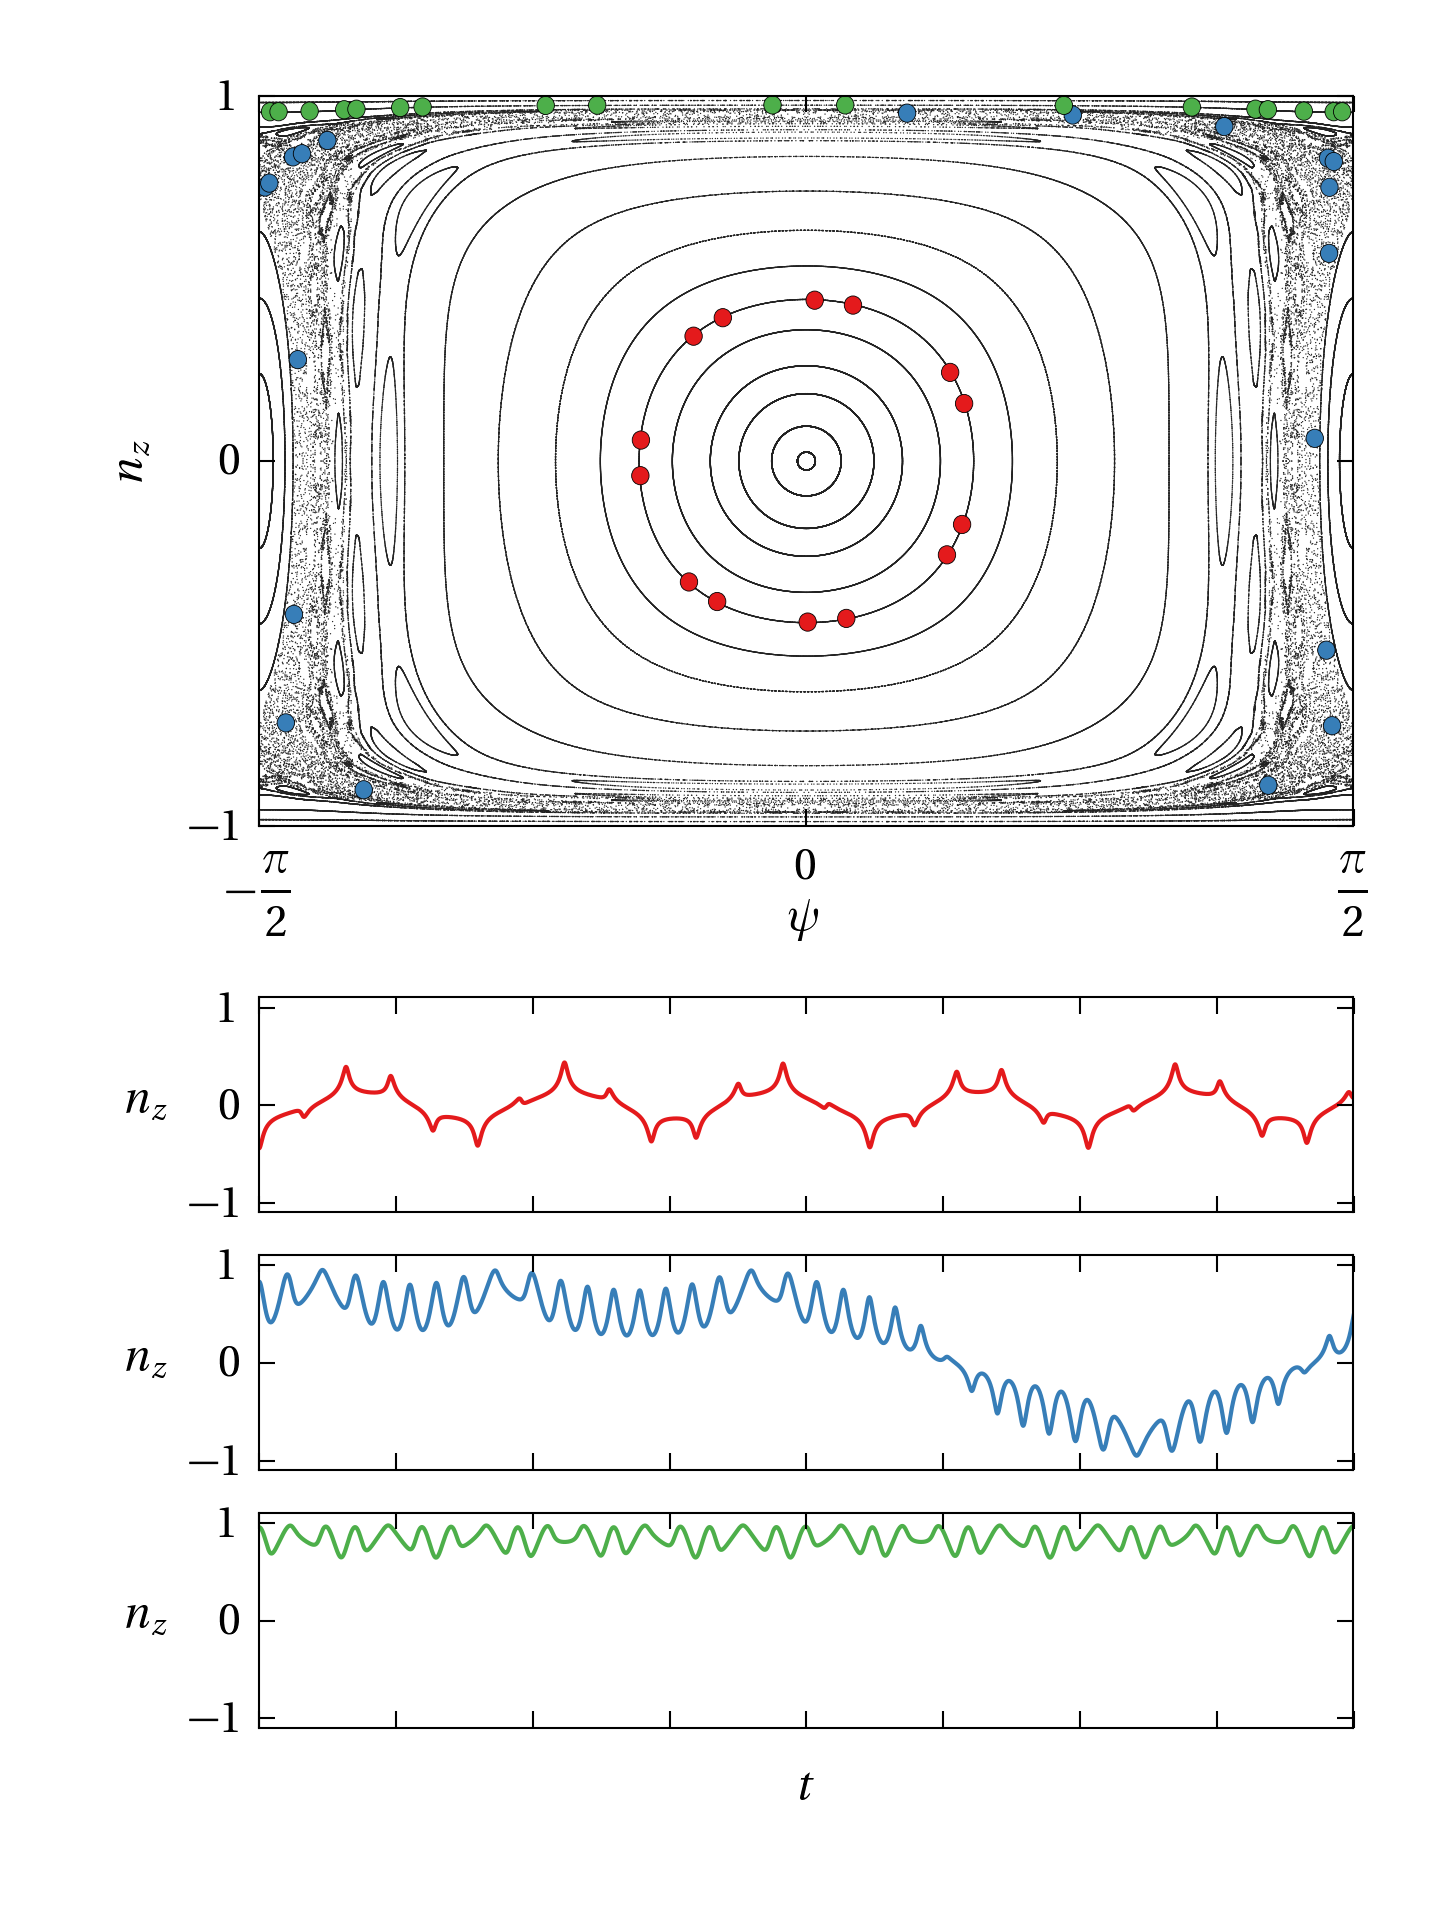
\includegraphics[width=12cm]{figs/poincare2o00.png}%
\caption{\label{fig:poincare2o00} Top: Poincar\'e surface-of-section of an axisymmetric particle with aspect ratios $\lambda=5$, $\kappa=2$. Bottom: Examples of what $n_z(t)$ looks like, given the trajectory indicated by the color coded markers on the surface-of-section. 
}
\end{figure}


The degeneracy of these solutions may be broken in the same way as discussed for axisymmetric particles in \Secref{jeffaxisymmetric}.

First, I expect the effect of particle and fluid inertia to make one or a few orbits preferred over the others, like in the axisymmetric case. \citet{lundell2011} show numerical simulations for $\Reys=0$ but $\st>0$ which support this expectation. The method used in Papers~A-D and Refs.~\cite{subramanian2005,subramanian2006} can in principle be extended to the case of ellipsoids. However, that calculation will involve large amounts of complicated algebra.

Second, thermal noise will kick the trajectories between different curves in the surface of section, analogous to the axisymmetric case. Eventually the initial condition is forgotten, and there is an orientational probability distribution over the space of all rotations. The distribution depends on the particle shape, and the strength of the noise. This is the topic of Paper~F, described further in \Secref{triaxialnoise} in Part II. In \Secref{orientationaldistributions} I introduce the concept of an orientational distribution more carefully.

\end{document}
